\chapter*{De Xi’an à Jiuzhaigou\markboth{De Xi’an à Jiuzhaigou}{}}
\section*{22 septembre 2015}
Avant de remonter sur le vélo, un peu de tourisme à Xi'an.

 D'abord la fameuse armée de terre cuite à quelques dizaines de km. Il y a 3 sites à visiter, le 1\ier\ est le plus petit.
\begin{center} 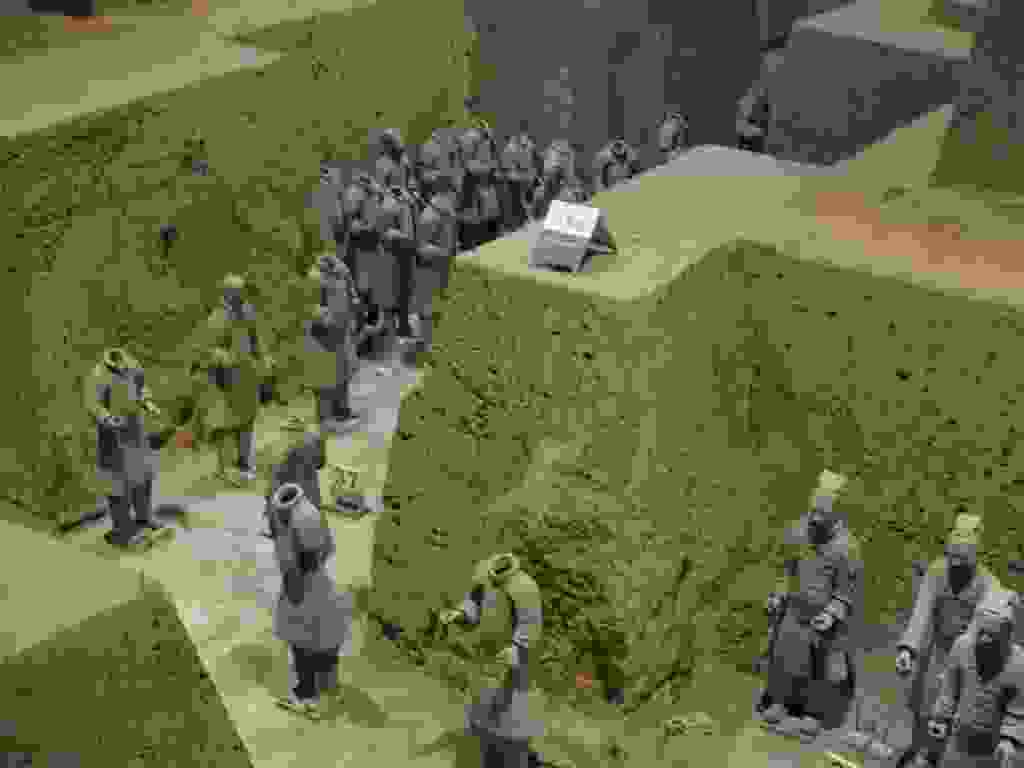
\includegraphics[width=\mywidth]{../wp-content/uploads/2015/09/wpid-wp-1442308836898-1024x768.jpg} \end{center}

\pagebreak
 Le 2\ieme\ est encore en cours de fouille.
\begin{center} 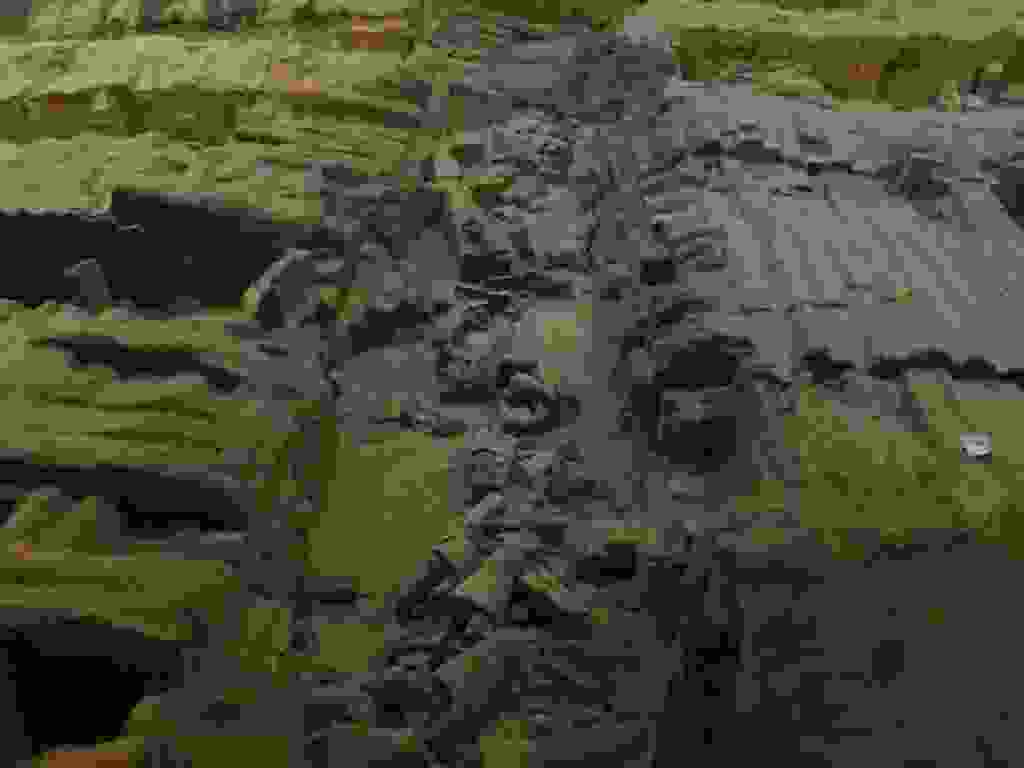
\includegraphics[width=\mywidth]{../wp-content/uploads/2015/09/wpid-wp-1442580768242-1024x768.jpg} \end{center}

 Enfin le dernier le plus spectaculaire.
\begin{center} 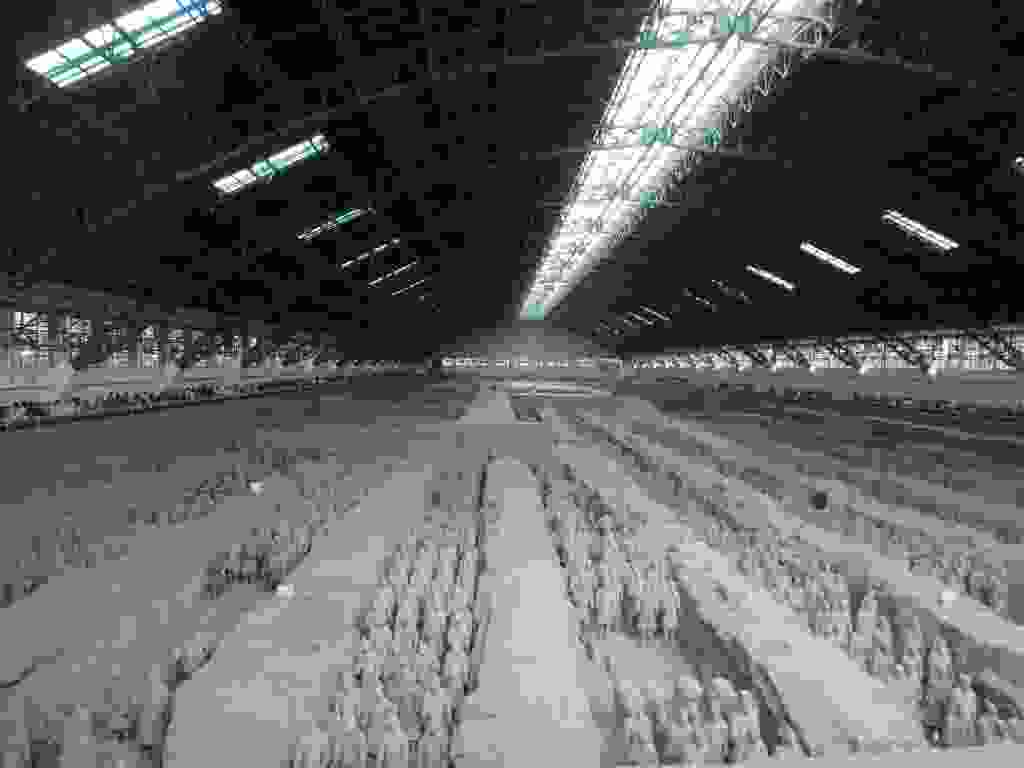
\includegraphics[width=\mywidth]{../wp-content/uploads/2015/09/wpid-wp-1442580502736-1024x768.jpg} \end{center}
 \begin{center} 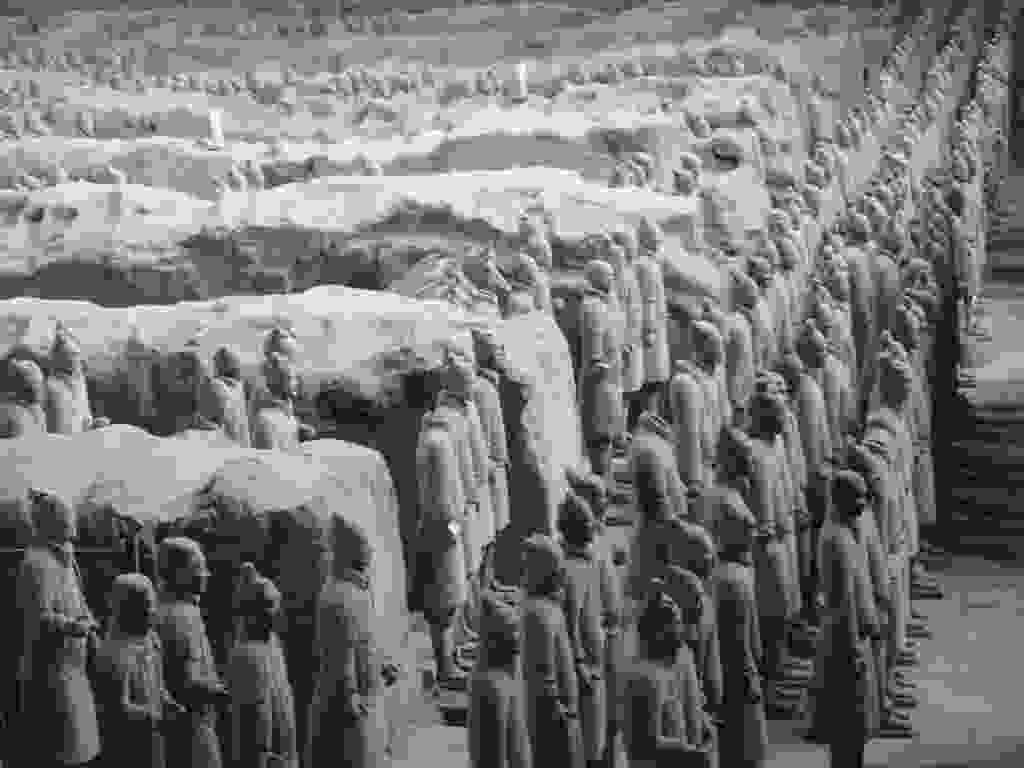
\includegraphics[width=\mywidth]{../wp-content/uploads/2015/09/wpid-wp-1442580568134-1024x768.jpg} \end{center}
\begin{center} 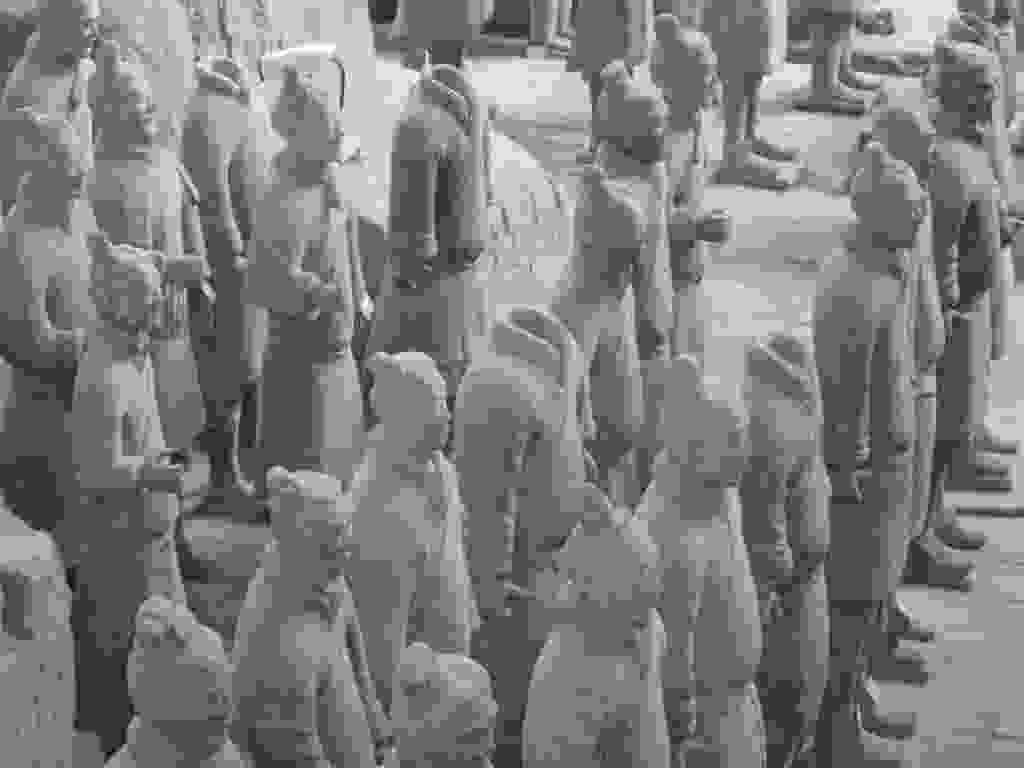
\includegraphics[width=\mywidth]{../wp-content/uploads/2015/09/wpid-wp-1442580602461-1024x768.jpg} \end{center}

\pagebreak
  Des soldats en cours de restauration.
\begin{center} 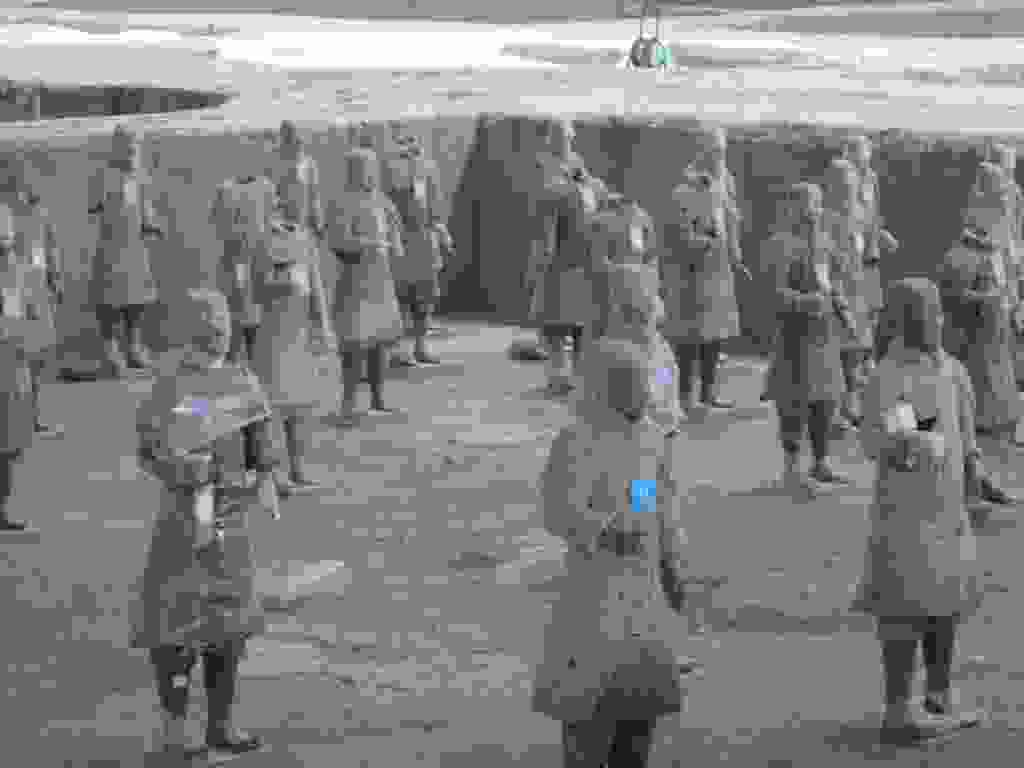
\includegraphics[width=\mywidth]{../wp-content/uploads/2015/09/wpid-wp-1442580709115-1024x768.jpg} \end{center}

 Xi'an est une ancienne cité chinoise située sur la route de la soie. Le centre est entouré de remparts.
\begin{center} 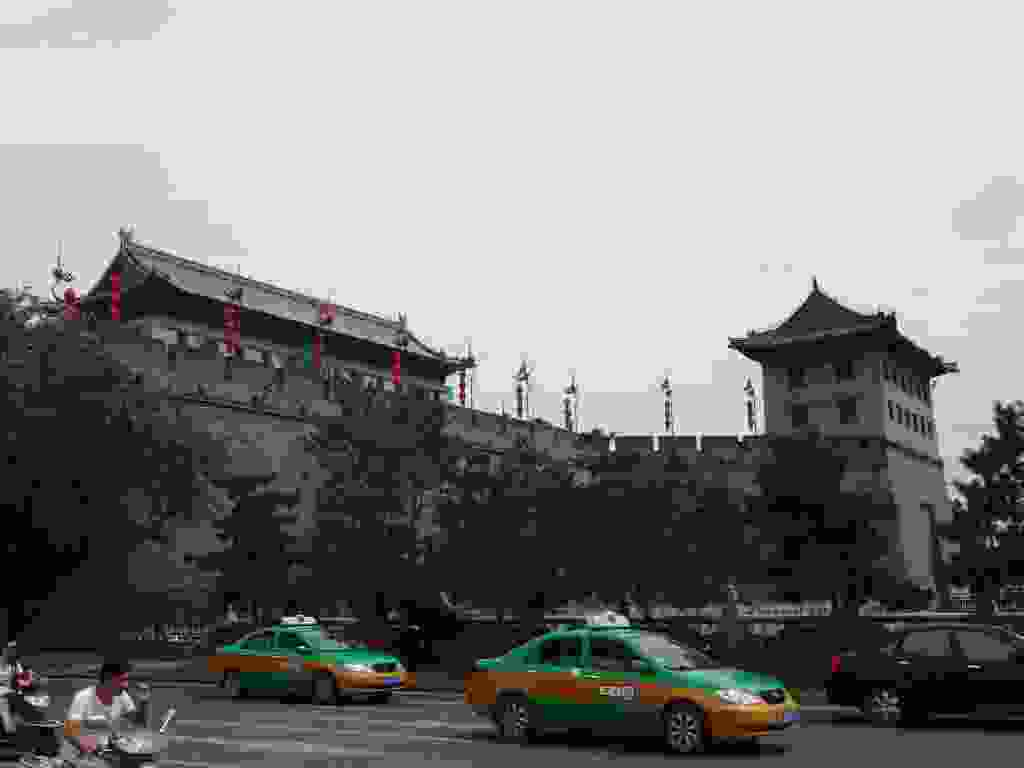
\includegraphics[width=\mywidth]{../wp-content/uploads/2015/09/wpid-wp-1442580873574-1024x768.jpg} \end{center}

\pagebreak
 La grande pagode de l'oie sauvage.
\begin{center} 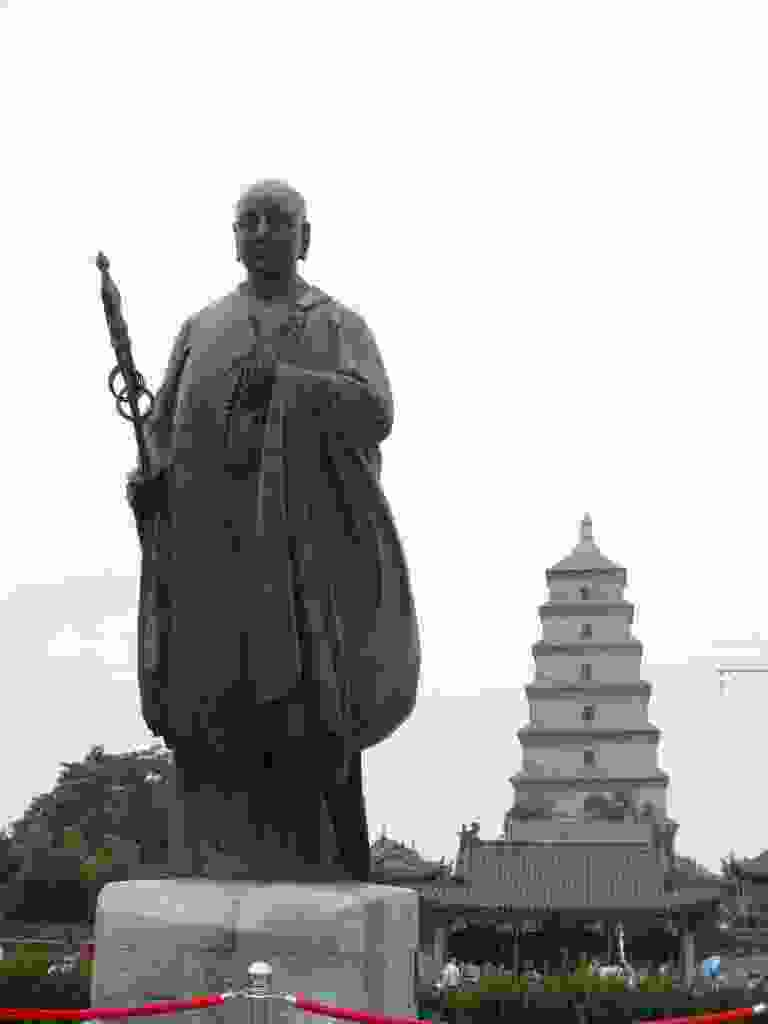
\includegraphics[height=0.83\textwidth]{../wp-content/uploads/2015/09/wpid-wp-1442308836897-e1442739534735-768x1024.jpg} \end{center}

 La Bell Tower.
\begin{center} 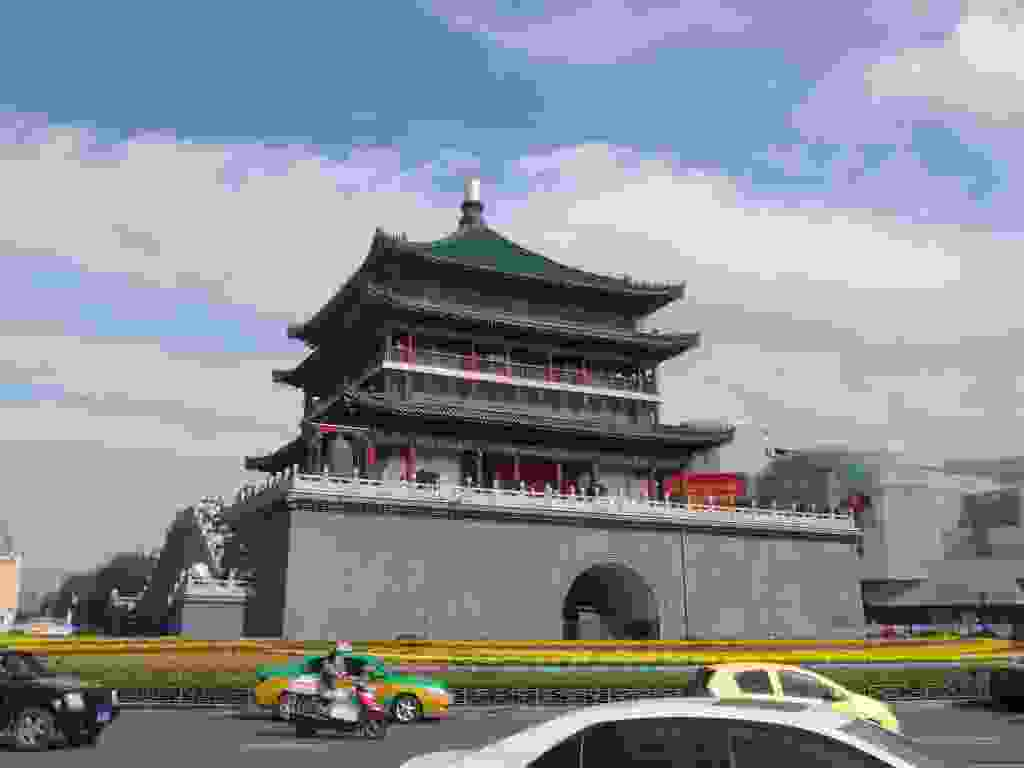
\includegraphics[width=\mywidth]{../wp-content/uploads/2015/09/wpid-wp-1442580997076-1024x768.jpg} \end{center}

 La Drum Tower. 
\begin{center} 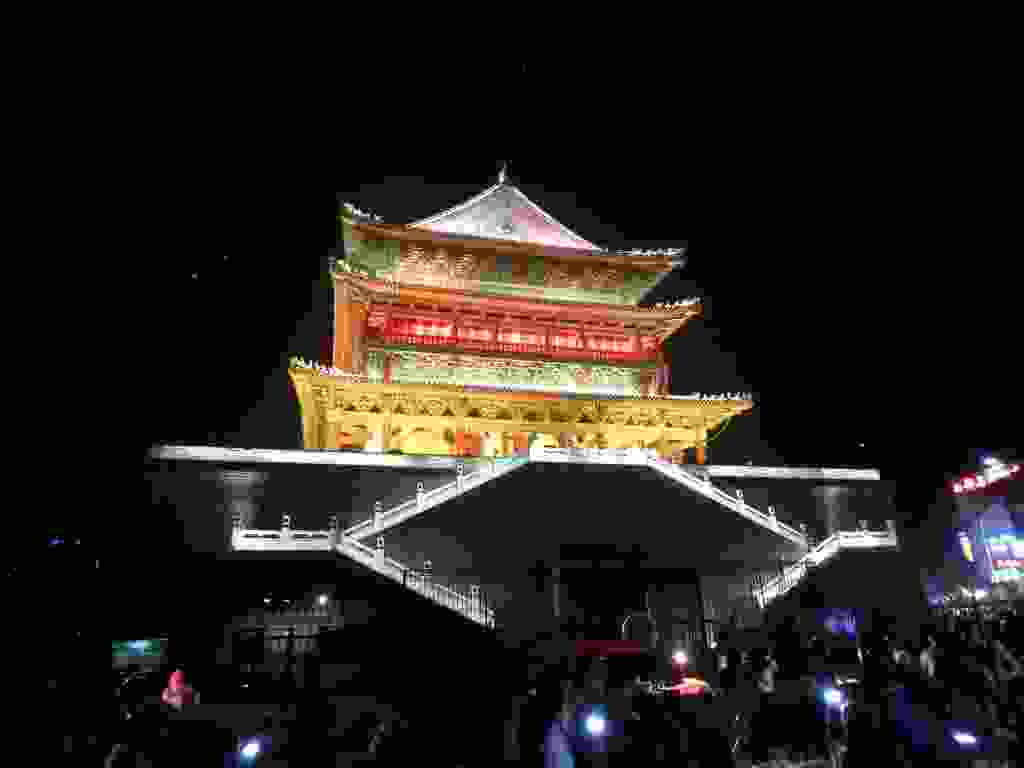
\includegraphics[width=\mywidth]{../wp-content/uploads/2015/09/wpid-wp-1442580837369-1024x768.jpg} \end{center}

 Le quartier musulman, très animé le jour comme la nuit.
\begin{center} 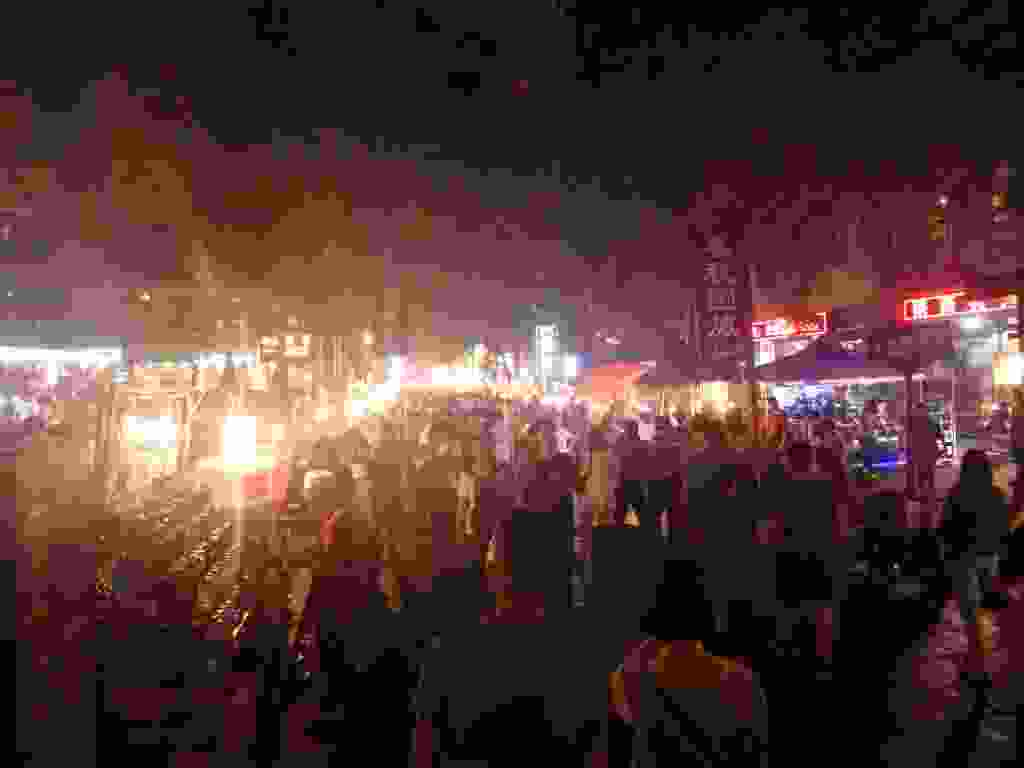
\includegraphics[width=\mywidth]{../wp-content/uploads/2015/09/P9046684-1024x768.jpg} \end{center}
\begin{center} 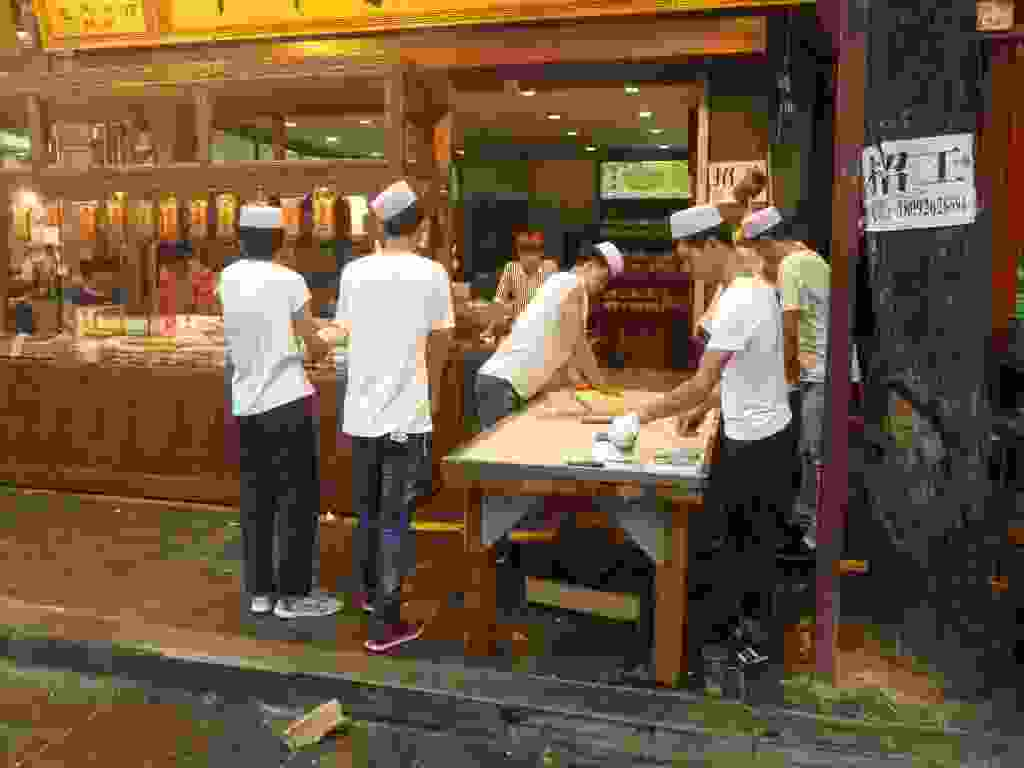
\includegraphics[width=\mywidth]{../wp-content/uploads/2015/09/wpid-wp-1442581025952-1024x768.jpg} \end{center}

 Dans les restaurants, les spécialités sont différents types de nouilles faites maison avec sauce épicée et souvent viande d'agneau. 
\begin{center} 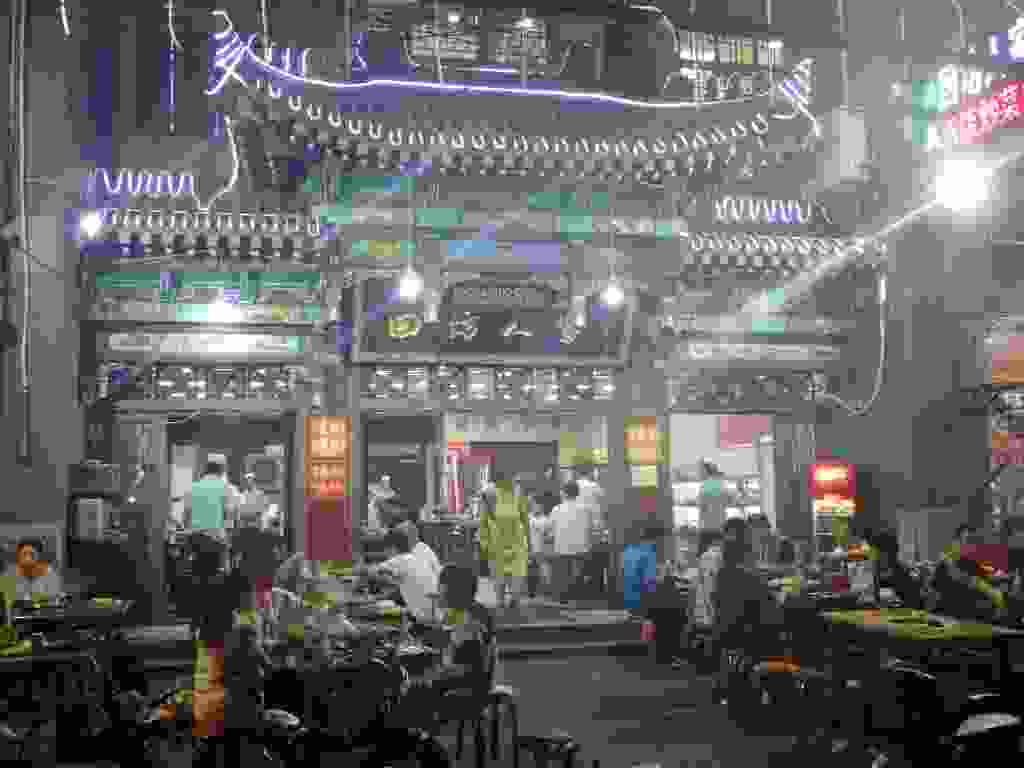
\includegraphics[width=\mywidth]{../wp-content/uploads/2015/09/P9046679-1024x768.jpg} \end{center}
\begin{center} 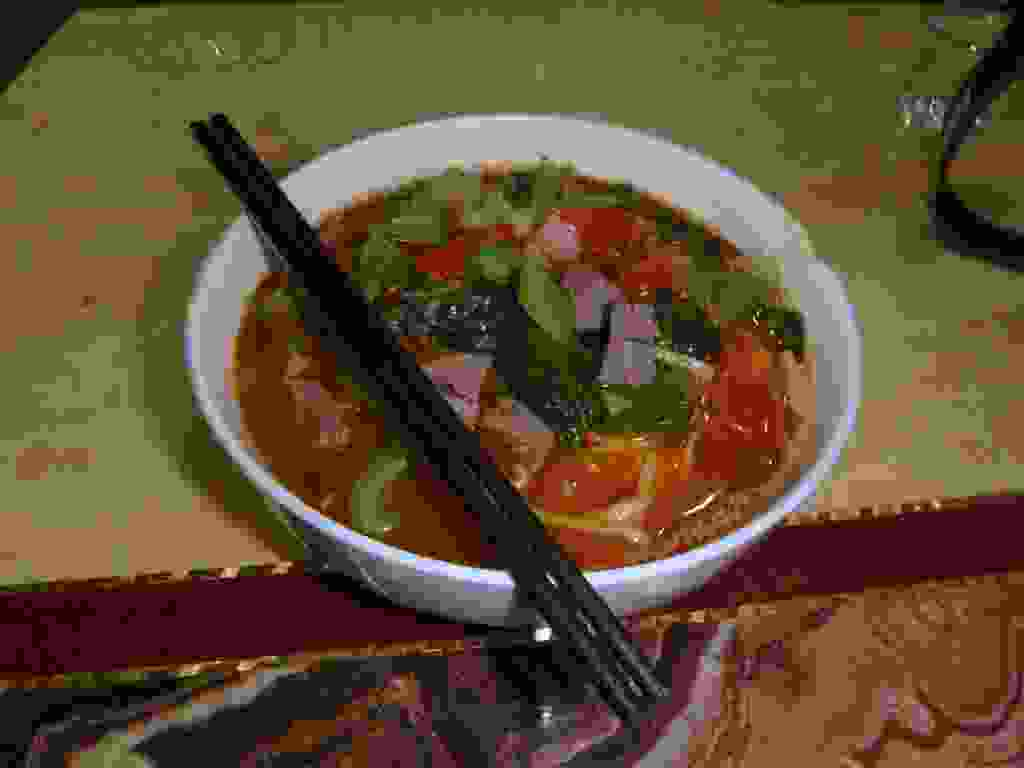
\includegraphics[width=\mywidth]{../wp-content/uploads/2015/09/P9046678-1024x768.jpg} \end{center}

 La grande mosquée.
\begin{center} 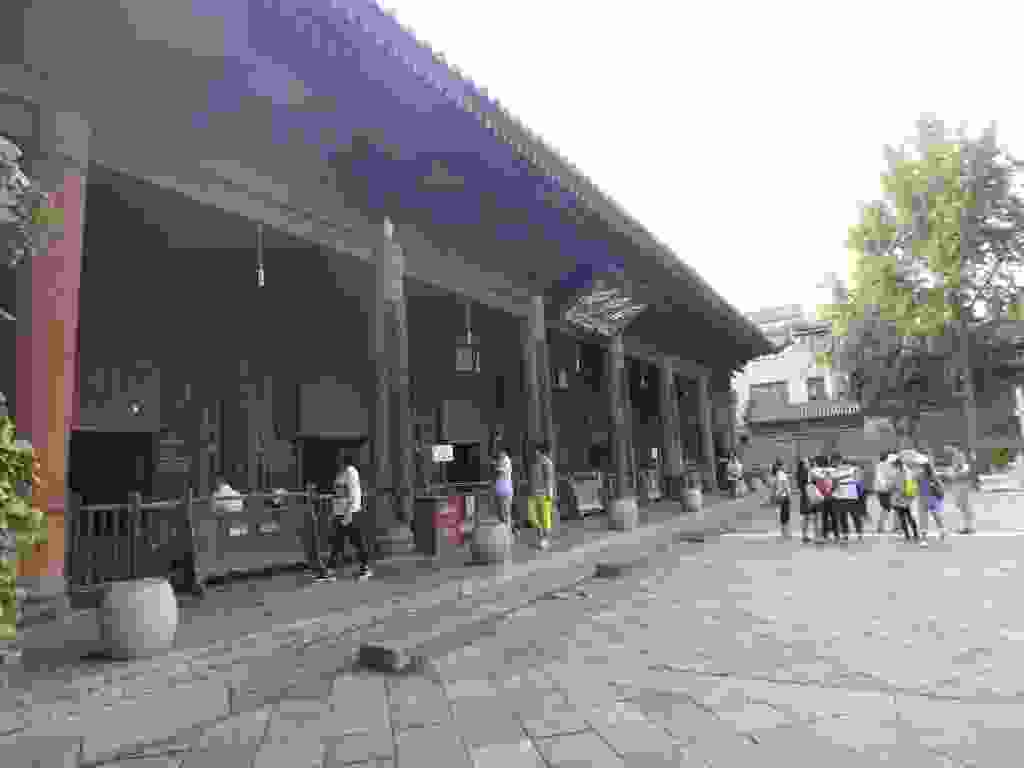
\includegraphics[width=\mywidth]{../wp-content/uploads/2015/09/wpid-wp-1442581072476-1024x768.jpg} \end{center}
\begin{center} 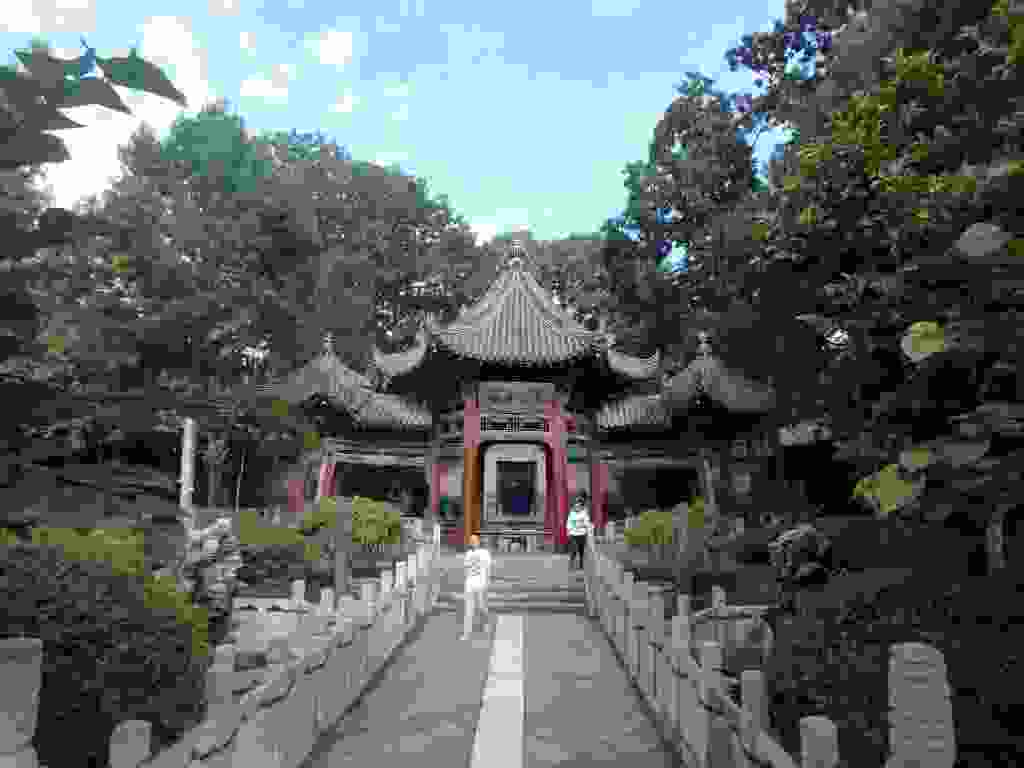
\includegraphics[width=\mywidth]{../wp-content/uploads/2015/09/wpid-wp-1442581100743-1024x768.jpg} \end{center}
 
 Le temple Wolong, je vois les moines en train de chanter. 
\begin{center} 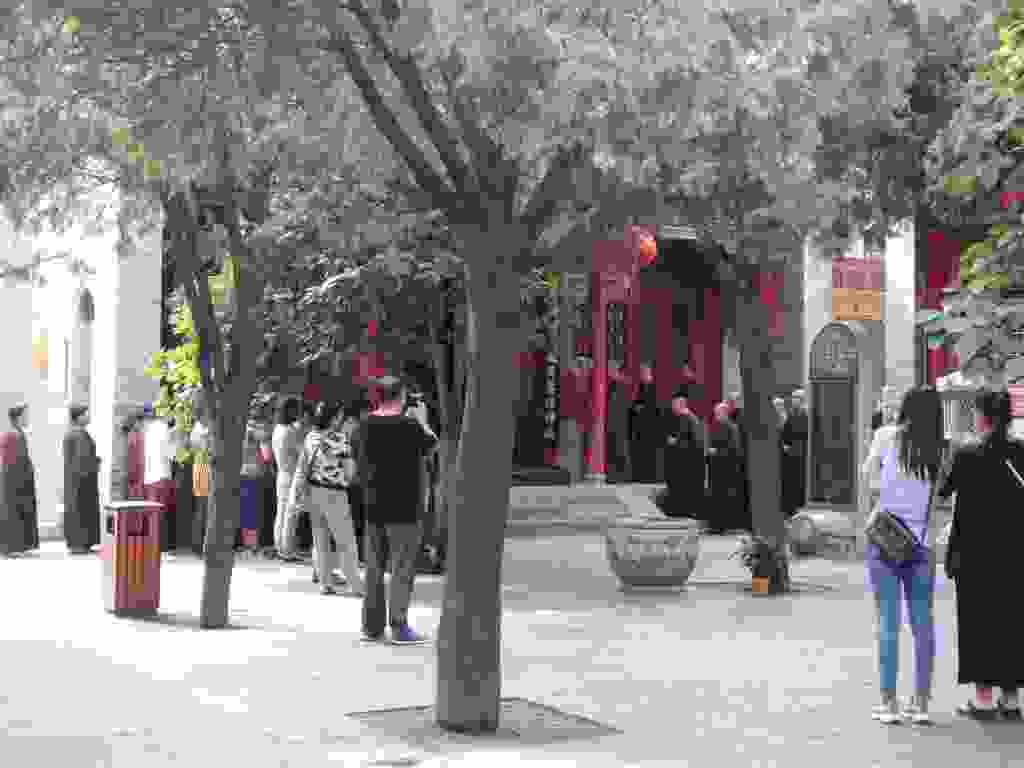
\includegraphics[width=\mywidth]{../wp-content/uploads/2015/09/wpid-wp-1442308836939-1024x768.jpg} \end{center}

\pagebreak
 Je quitte Xi'an vers l'ouest pour 9 jours de vélo jusqu'à Jiuzhaigou. Premières impressions : ça roule n'importe comment mais assez lentement, j'ai le temps de voir venir.

 Pour sortir de la ville, quelques pistes cyclables utilisées par les scooters électriques et les velib.
\begin{center} 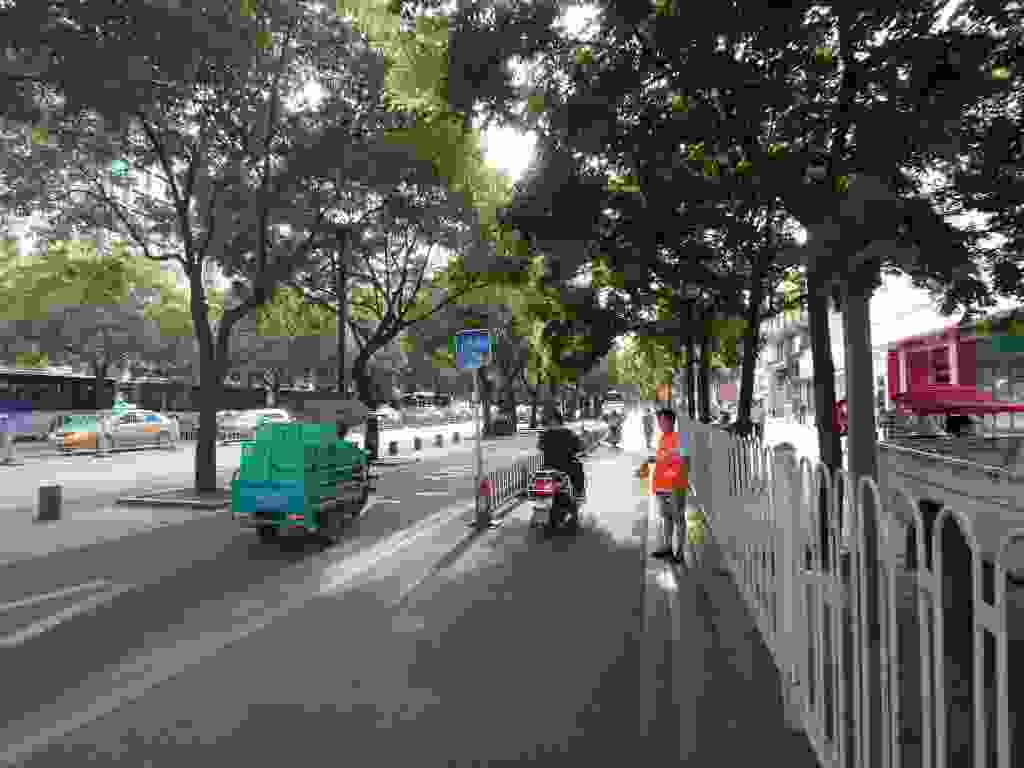
\includegraphics[width=\mywidth]{../wp-content/uploads/2015/09/wpid-wp-1442581159940-1024x768.jpg} \end{center}
\begin{center} 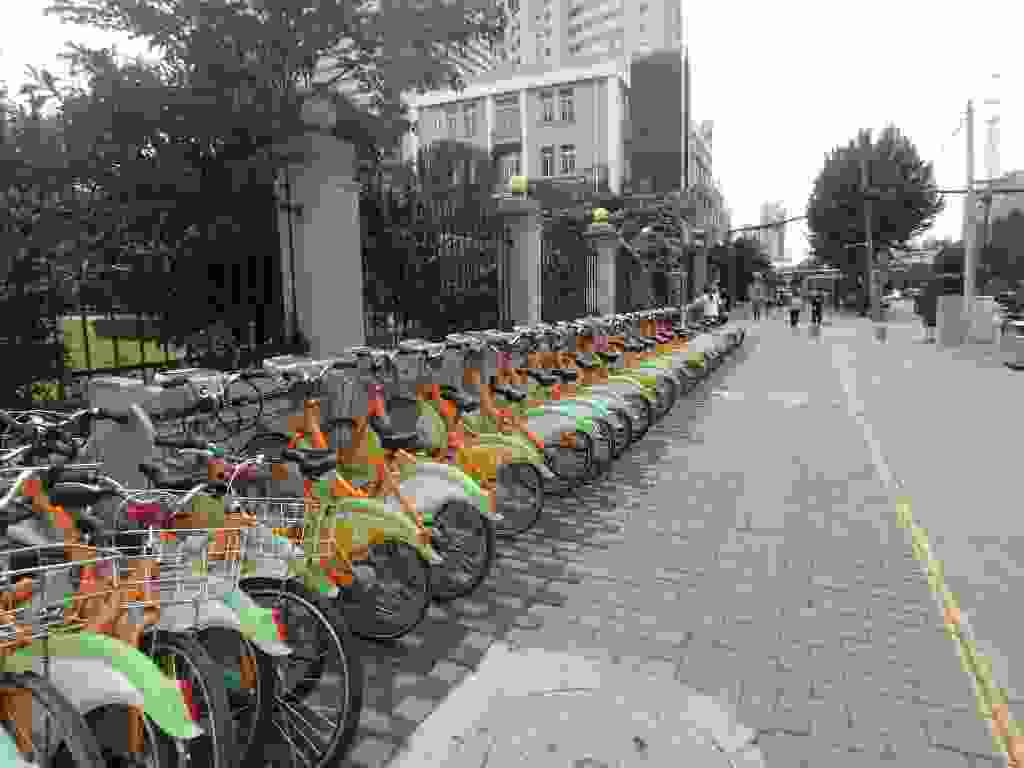
\includegraphics[width=\mywidth]{../wp-content/uploads/2015/09/wpid-wp-1442308836863-1024x768.jpg} \end{center}

\pagebreak
 2 jours de plat pour commencer, au milieu des champs et des usines.
\begin{center} 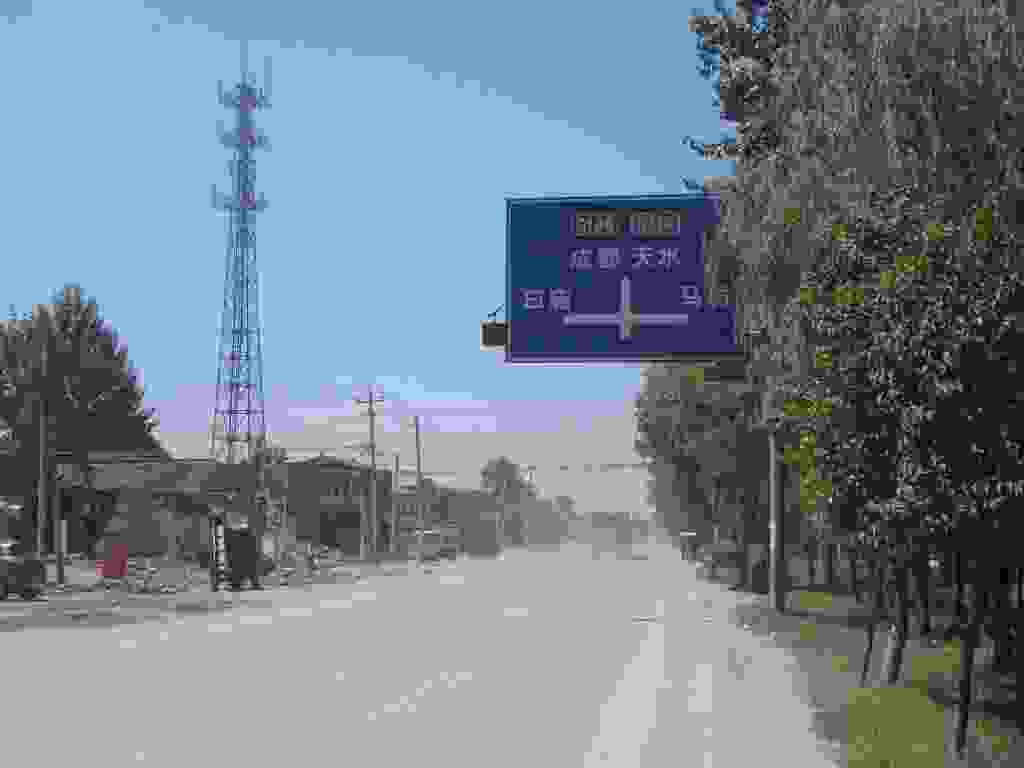
\includegraphics[width=\mywidth]{../wp-content/uploads/2015/09/wpid-p9066732-1024x768.jpg} \end{center}

 Puis les cols s'enchaînent ainsi que 3 jours de pluie, quelques rares moments pour apprécier le paysage.
\begin{center} 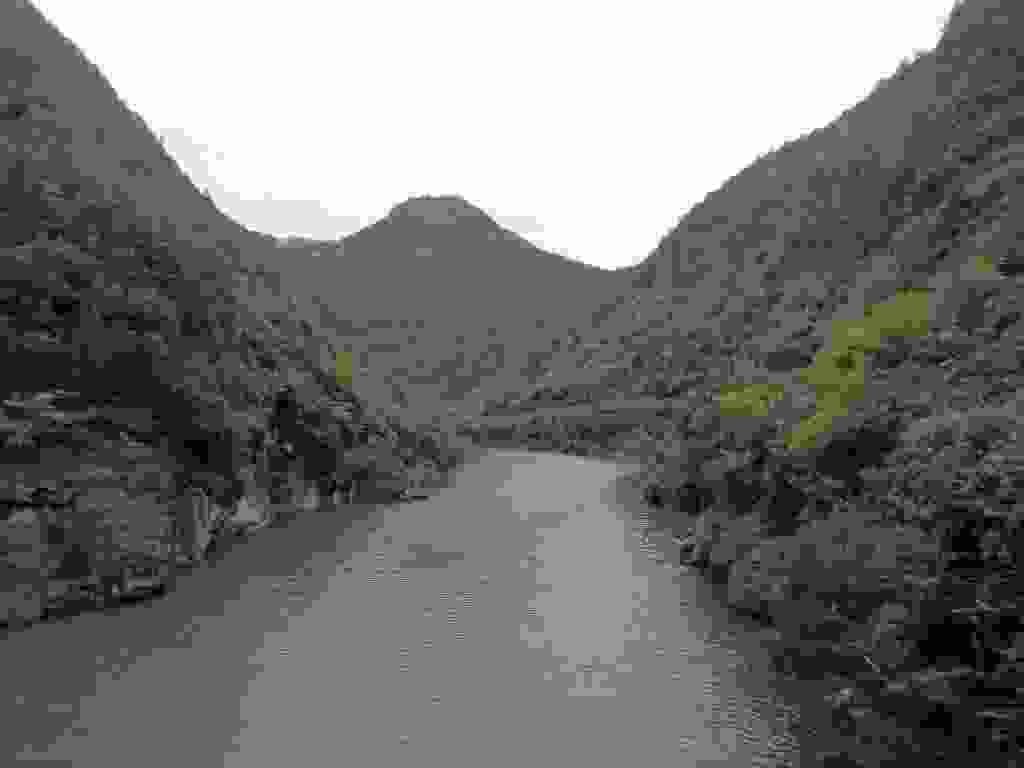
\includegraphics[width=\mywidth]{../wp-content/uploads/2015/09/wpid-p9096768-1024x768.jpg} \end{center}
\begin{center} 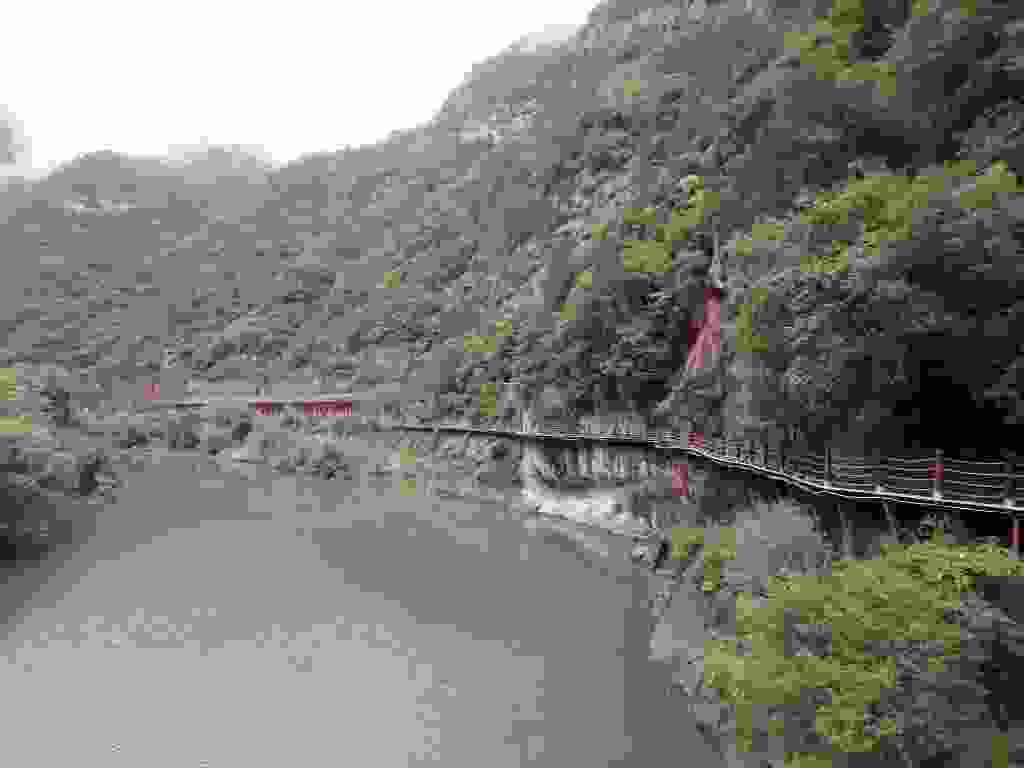
\includegraphics[width=\mywidth]{../wp-content/uploads/2015/09/wpid-p9096769-1024x768.jpg} \end{center}
\begin{center} 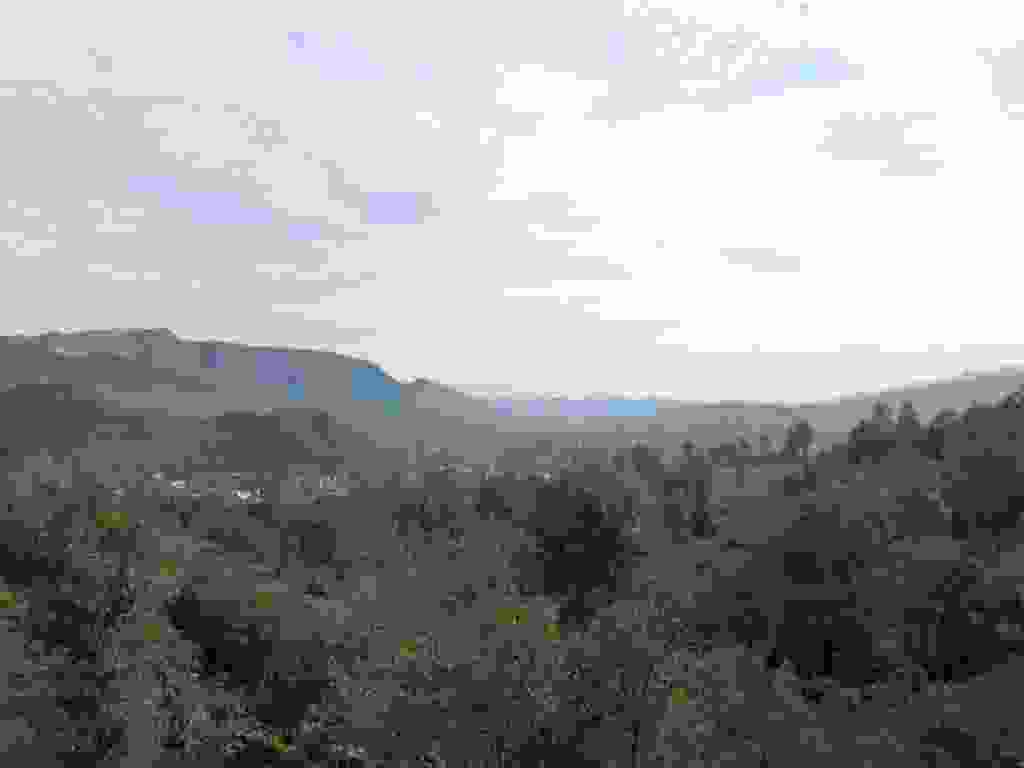
\includegraphics[width=\mywidth]{../wp-content/uploads/2015/09/wpid-p9116786-1024x768.jpg} \end{center}
\begin{center} 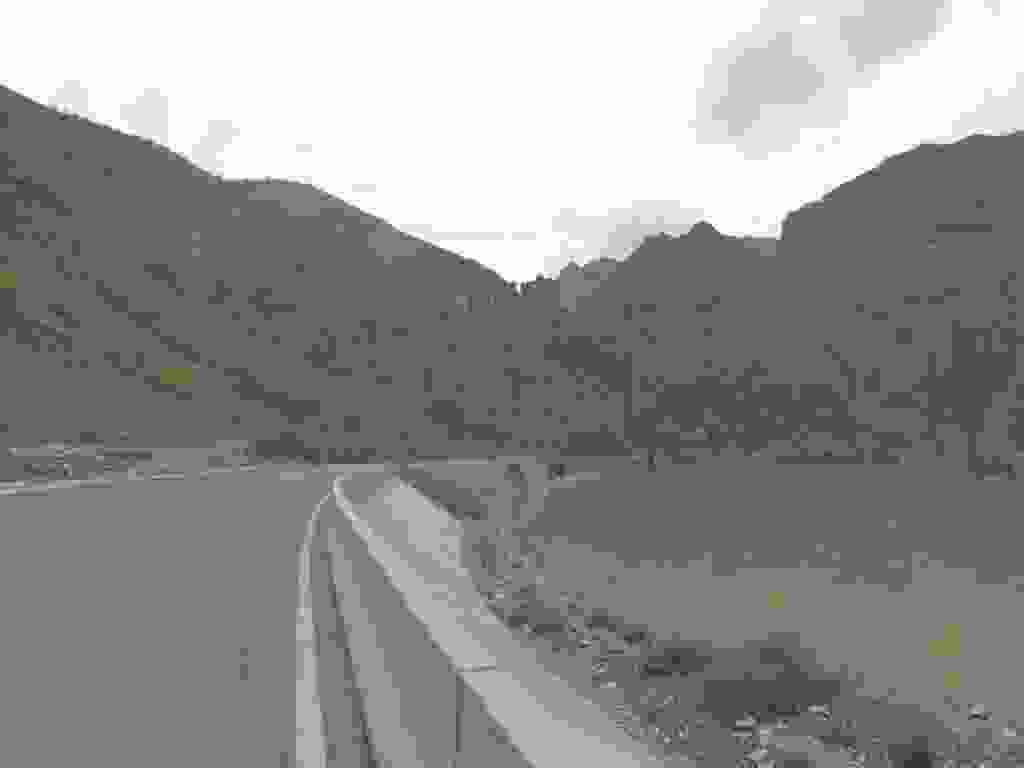
\includegraphics[width=\mywidth]{../wp-content/uploads/2015/09/wpid-p9126807-1024x768.jpg} \end{center}

 J'alterne camping et hôtel, pas facile à identifier dans les villages.
\begin{center} 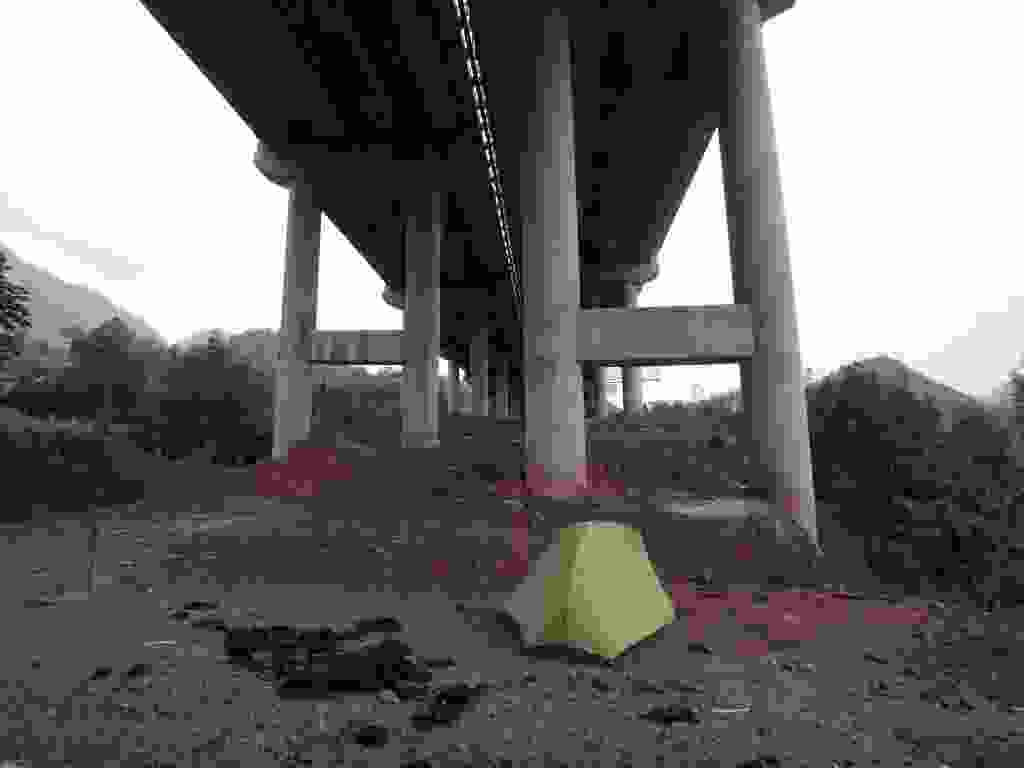
\includegraphics[width=\mywidth]{../wp-content/uploads/2015/09/wpid-p9106784-1024x768.jpg} \end{center}

\pagebreak
 Les villes sont modernes avec des grands immeubles en construction partout.
\begin{center} 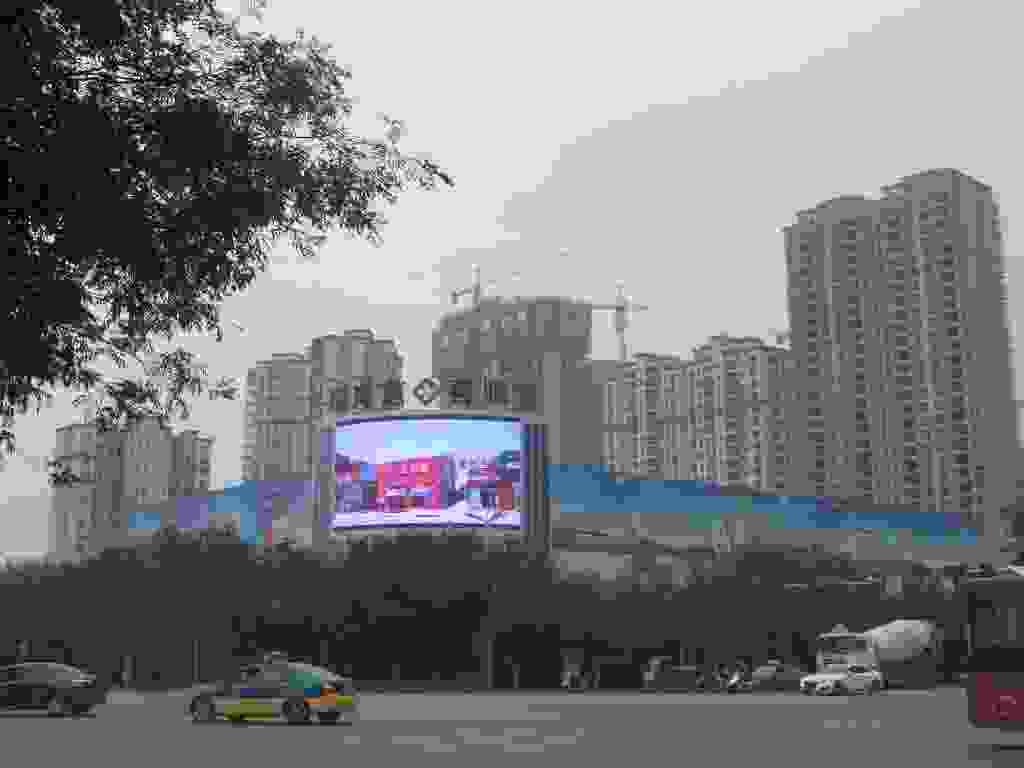
\includegraphics[width=\mywidth]{../wp-content/uploads/2015/09/P9076744-1024x768.jpg} \end{center}
\begin{center} 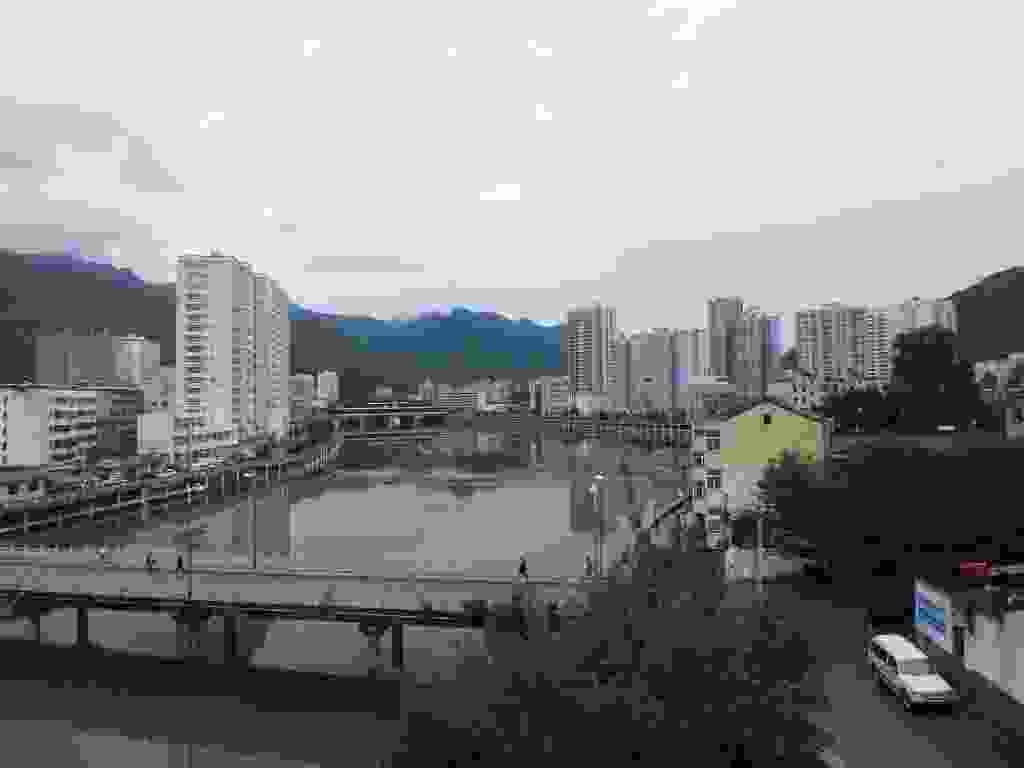
\includegraphics[width=\mywidth]{../wp-content/uploads/2015/09/wpid-p9096761-1024x768.jpg} \end{center}
\begin{center} 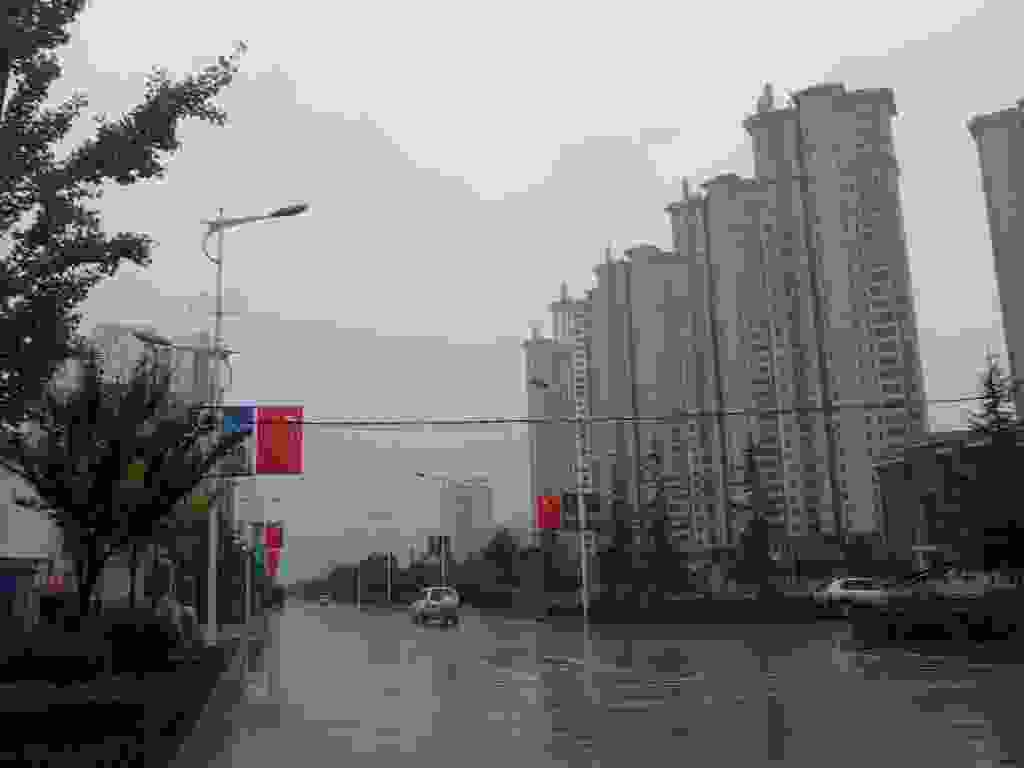
\includegraphics[width=\mywidth]{../wp-content/uploads/2015/09/P9106779-1024x768.jpg} \end{center}

 Les villages semblent beaucoup moins développés.
\begin{center} 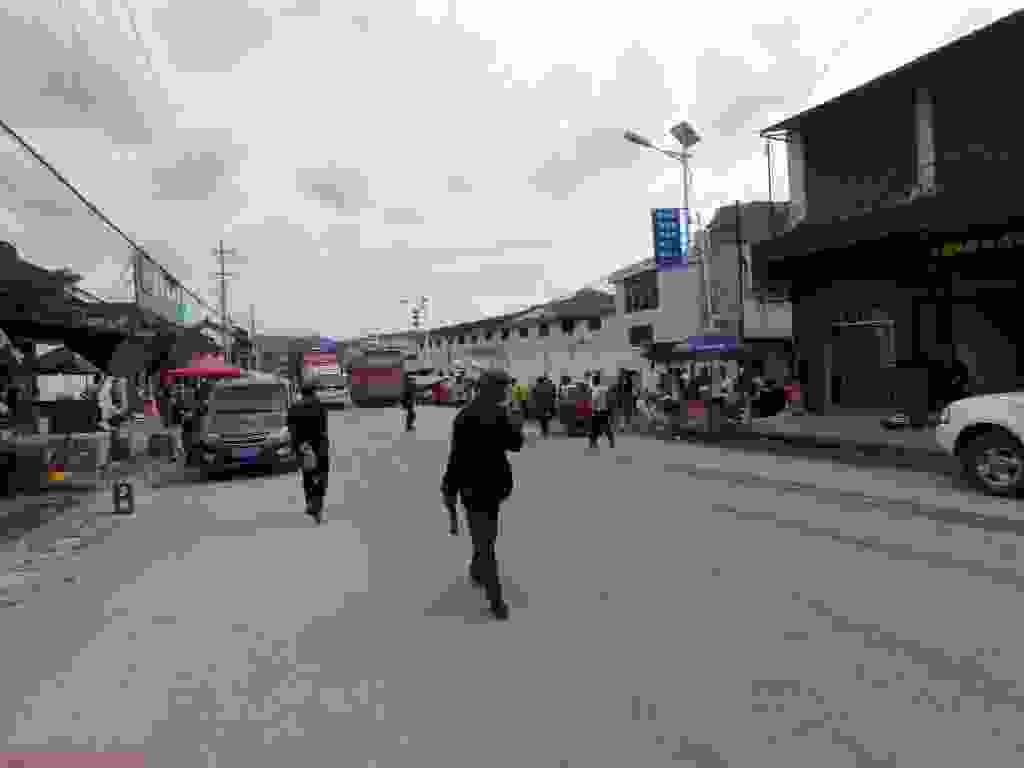
\includegraphics[width=\mywidth]{../wp-content/uploads/2015/09/wpid-p9116788-1024x768.jpg} \end{center}

\pagebreak
 Plusieurs temples le long de la route.
\begin{center} 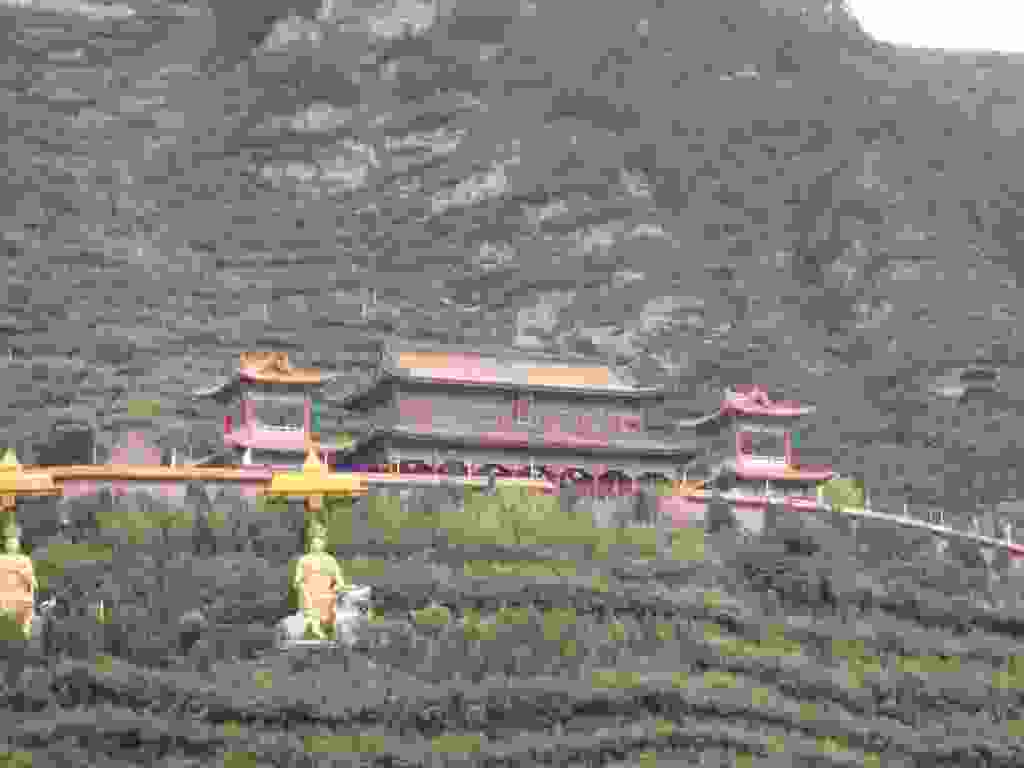
\includegraphics[width=\mywidth]{../wp-content/uploads/2015/09/wpid-wp-1442581295173-1024x768.jpg} \end{center}
\begin{center} 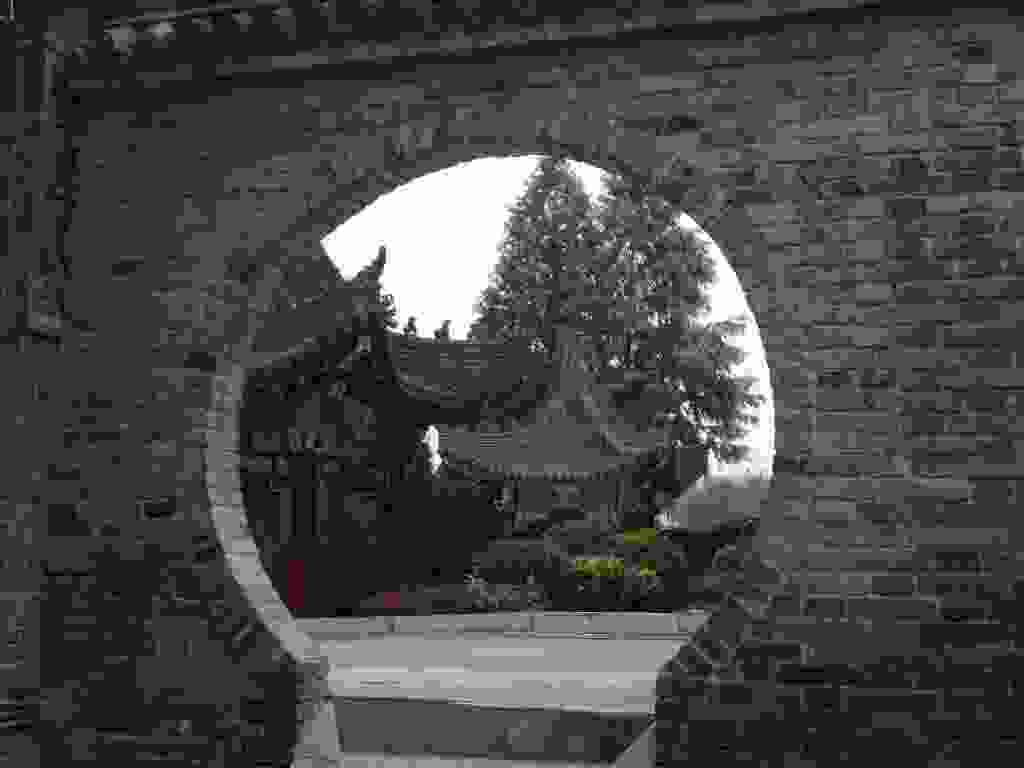
\includegraphics[width=\mywidth]{../wp-content/uploads/2015/09/P9076737-1024x768.jpg} \end{center}

\pagebreak
 Peu de trafic sur certaines portions qui longent l'autoroute toute neuve.
\begin{center} 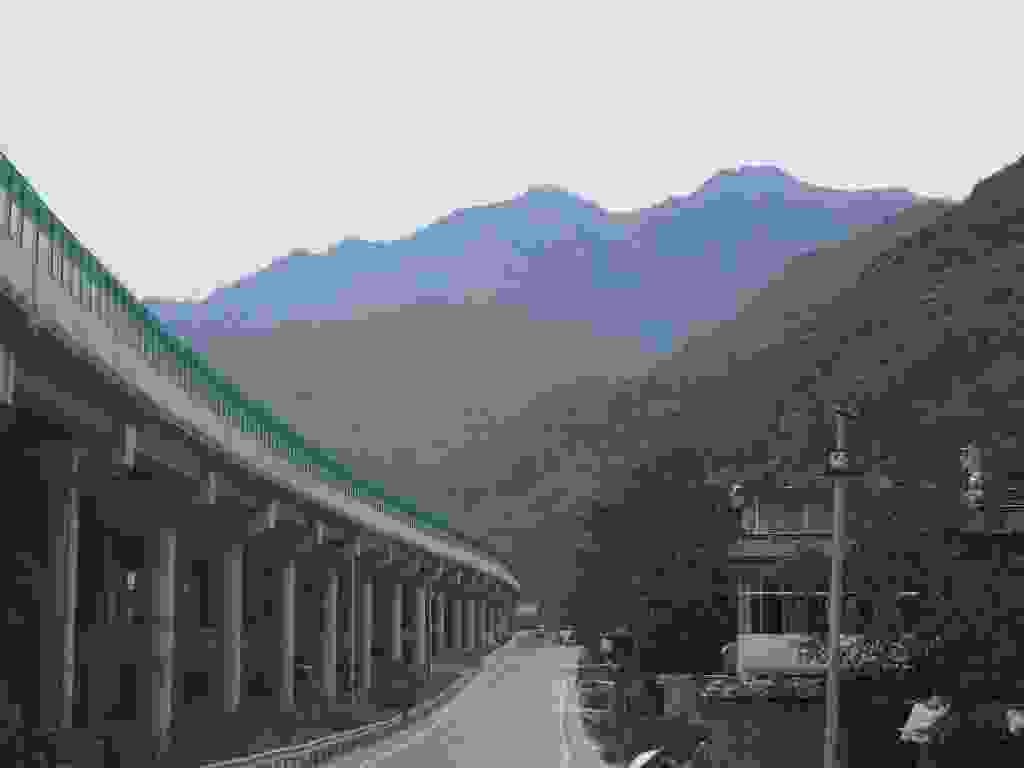
\includegraphics[width=\mywidth]{../wp-content/uploads/2015/09/wpid-p9116795-1024x768.jpg} \end{center}

 Je m'arrête dans un village, un homme m'aide à chercher un hôtel puis finalement m'invite à passer la nuit chez lui.
\begin{center} 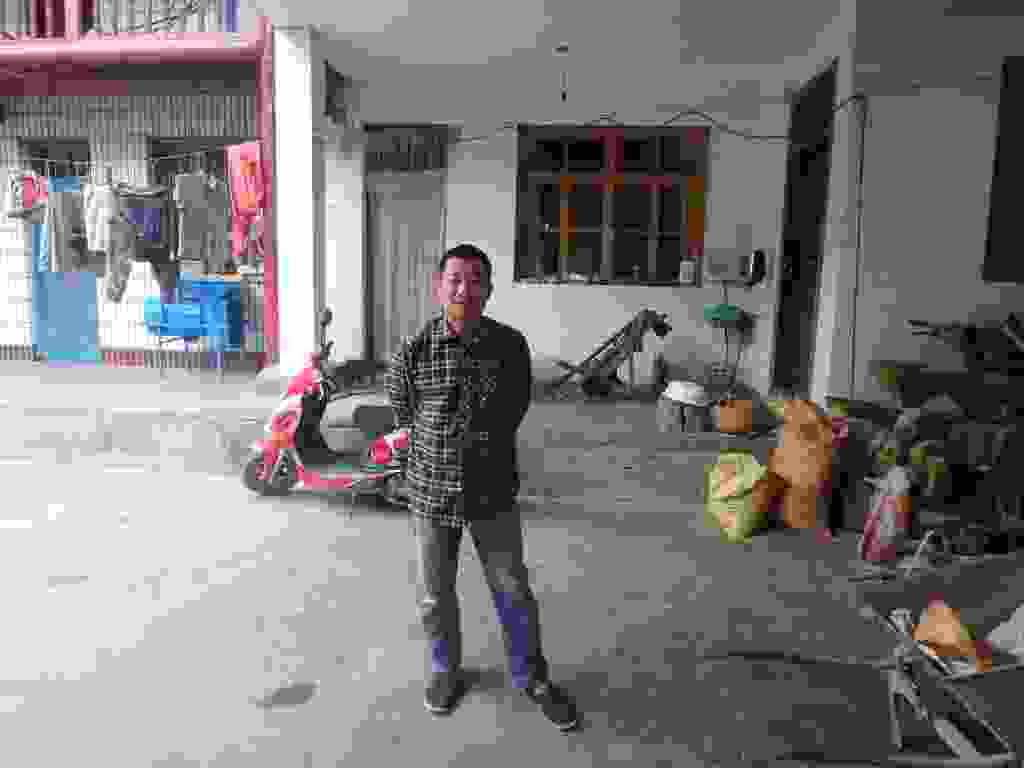
\includegraphics[width=\mywidth]{../wp-content/uploads/2015/09/wpid-p9136835-1024x768.jpg} \end{center}

\pagebreak
 Les enfants sont tout fous quand je leur montre les photos que je prends d'eux.
\begin{center} 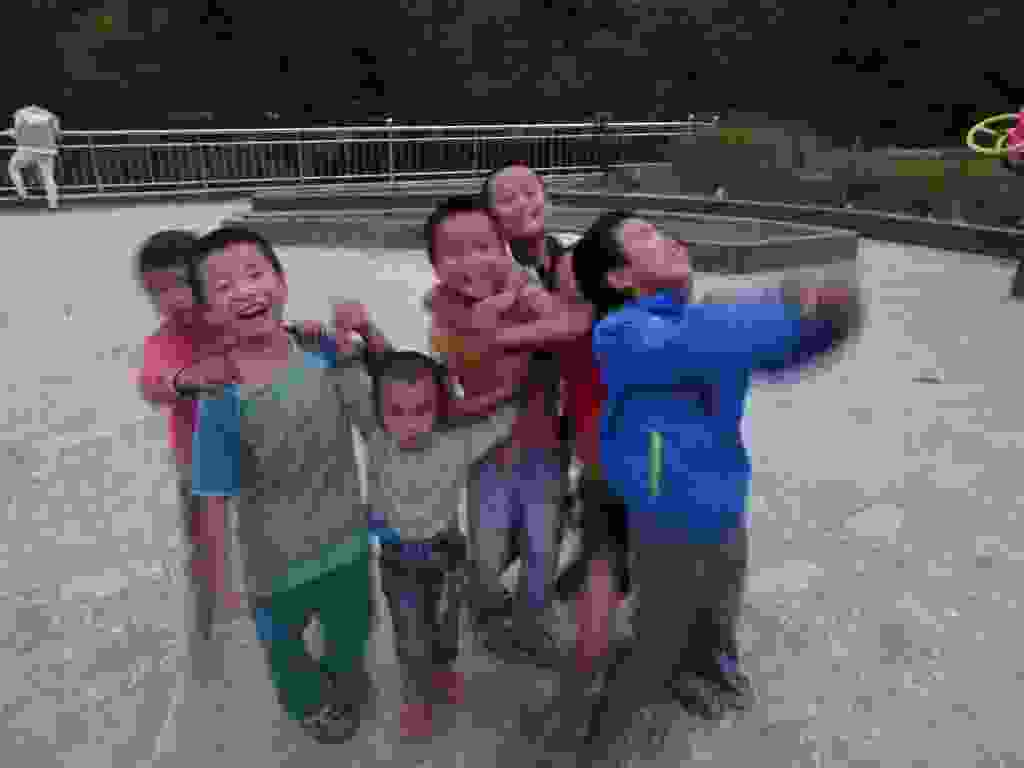
\includegraphics[width=\mywidth]{../wp-content/uploads/2015/09/wpid-p9126823-1024x768.jpg} \end{center}
\begin{center} 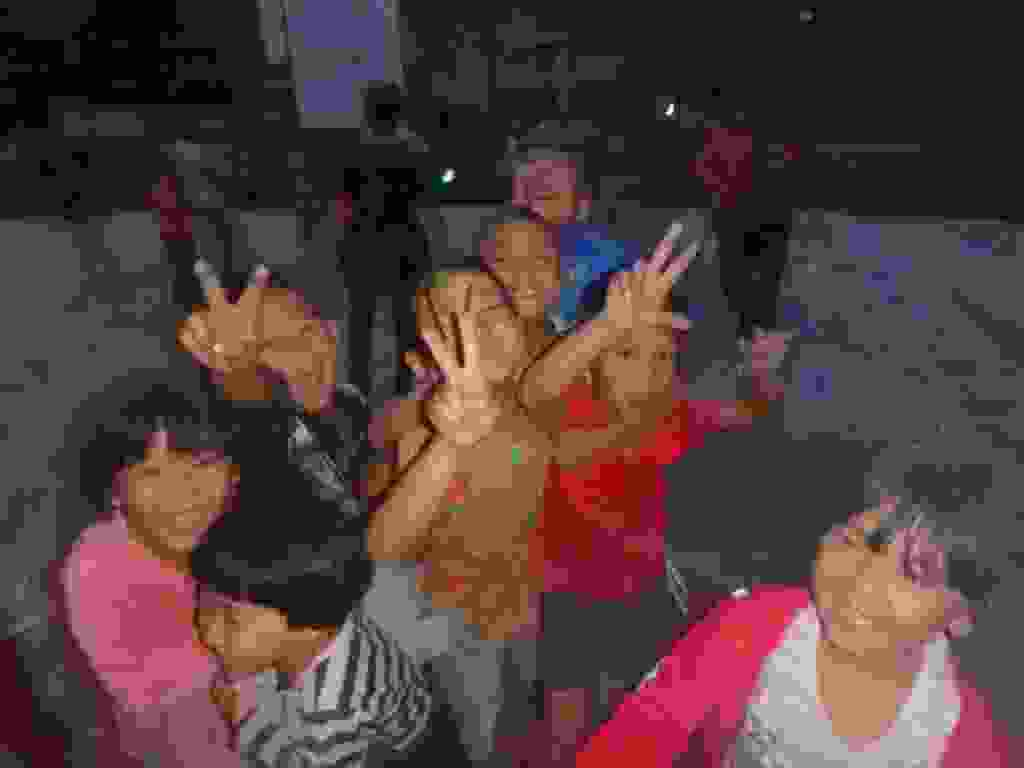
\includegraphics[width=\mywidth]{../wp-content/uploads/2015/09/wpid-p9126826-1024x768.jpg} \end{center}

\pagebreak
 Malgré la communication difficile, je suis bien accueilli dans les restaurants et parfois on refuse de me faire payer l'addition. 
\begin{center} 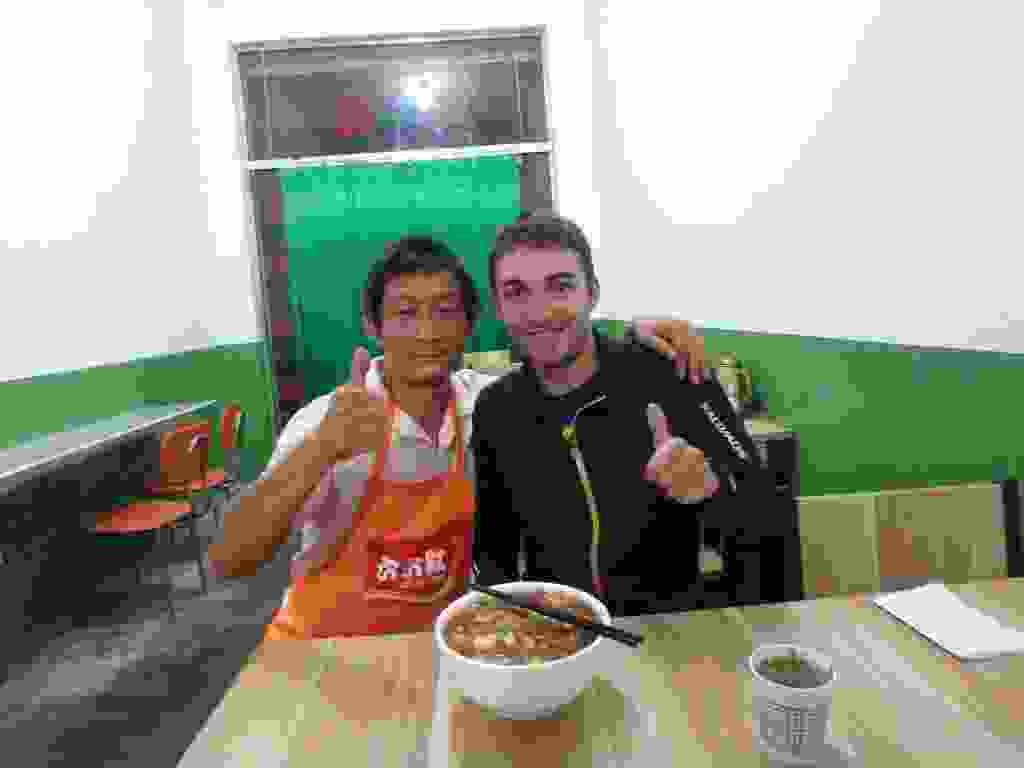
\includegraphics[width=\mywidth]{../wp-content/uploads/2015/09/wpid-p9096774-1024x768.jpg} \end{center}
\begin{center} 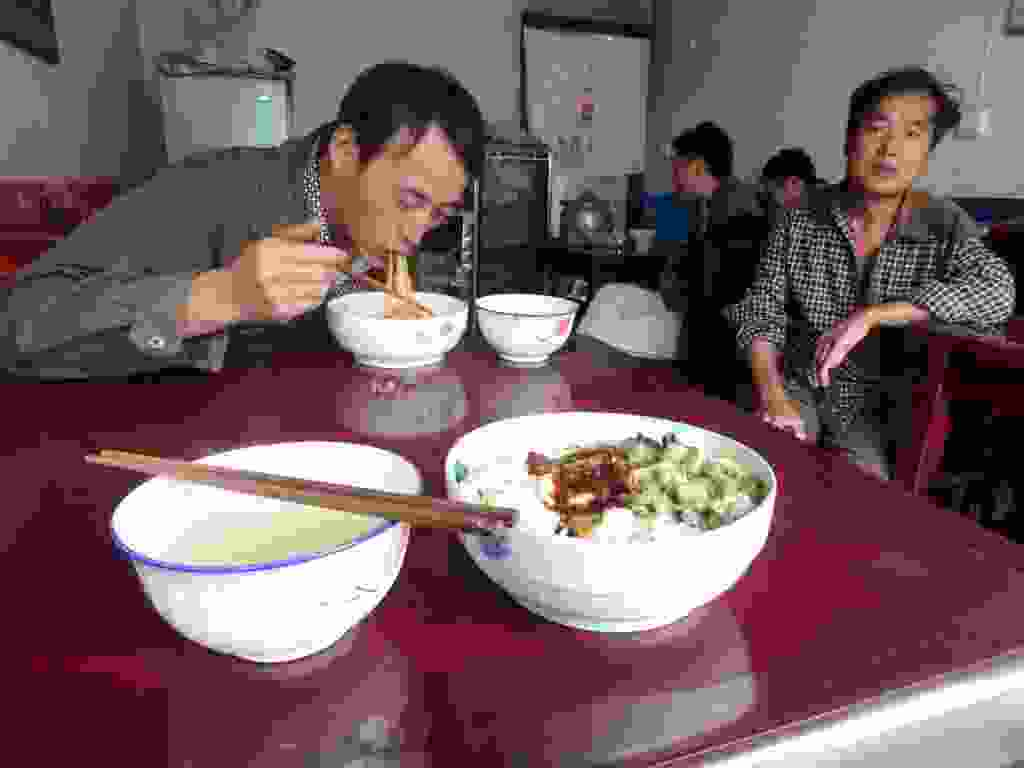
\includegraphics[width=\mywidth]{../wp-content/uploads/2015/09/wpid-p9096762-1024x768.jpg} \end{center}

\pagebreak
  Les cols deviennent de plus en plus long en approchant de Jiuzhaigou. 
\begin{center} 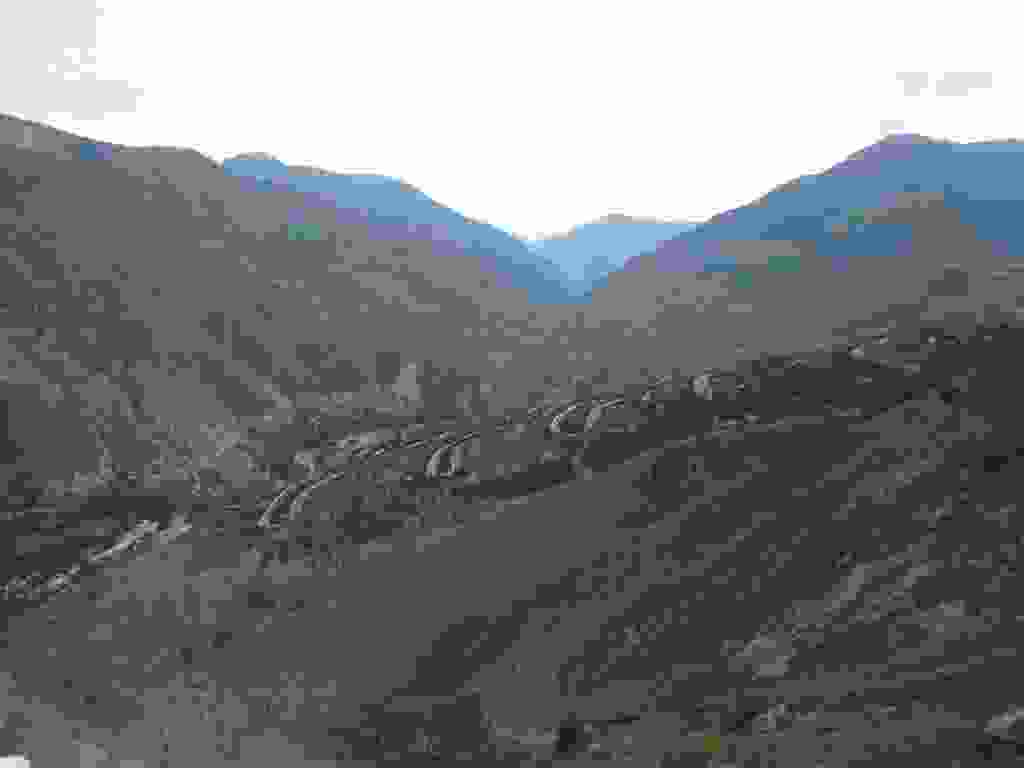
\includegraphics[width=\mywidth]{../wp-content/uploads/2015/09/wpid-p9136840-1024x768.jpg} \end{center}
\begin{center} 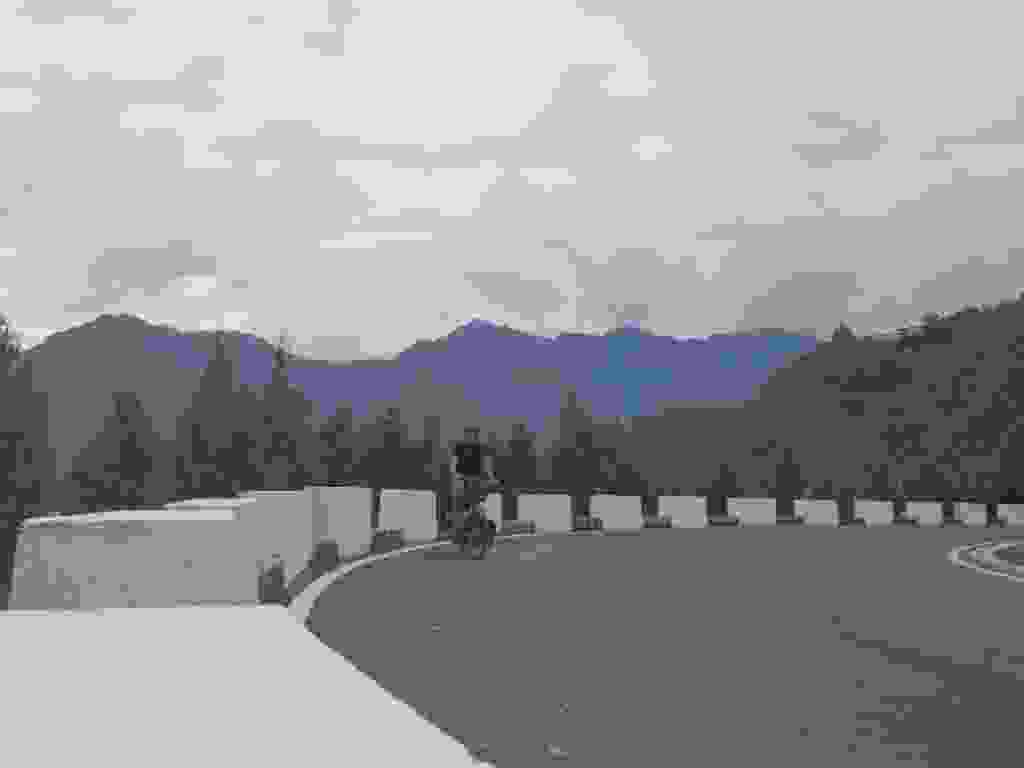
\includegraphics[width=\mywidth]{../wp-content/uploads/2015/09/wpid-p9136842-1024x768.jpg} \end{center}
\begin{center} 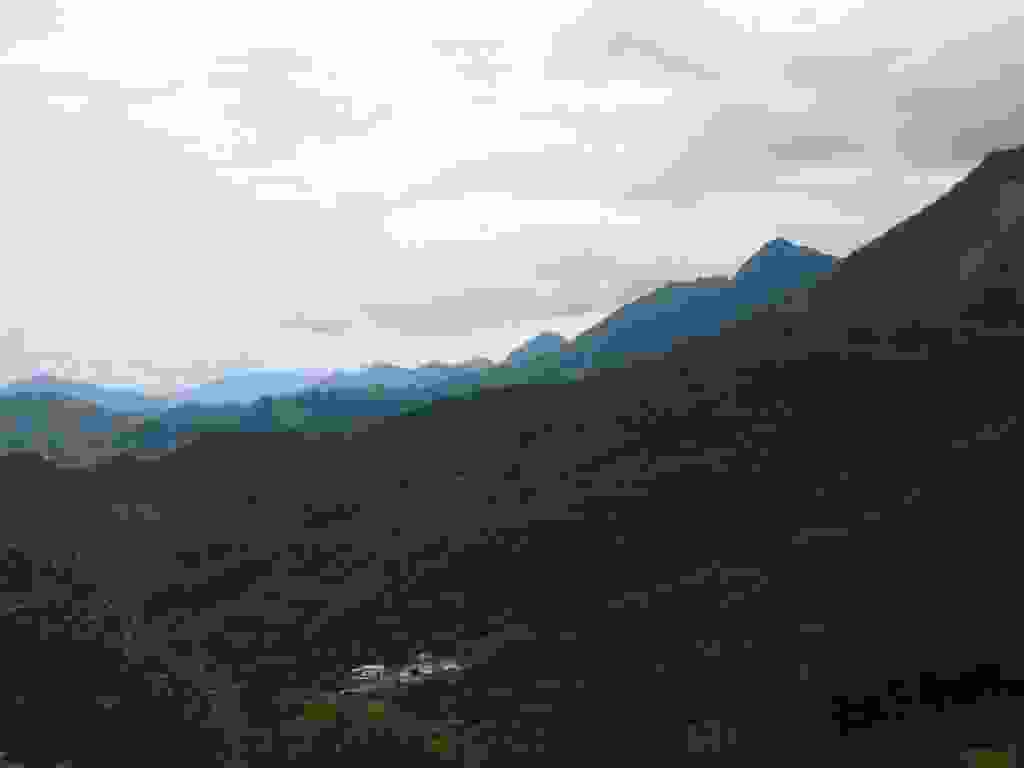
\includegraphics[width=\mywidth]{../wp-content/uploads/2015/09/wpid-p9136850-1024x768.jpg} \end{center}
\begin{center} 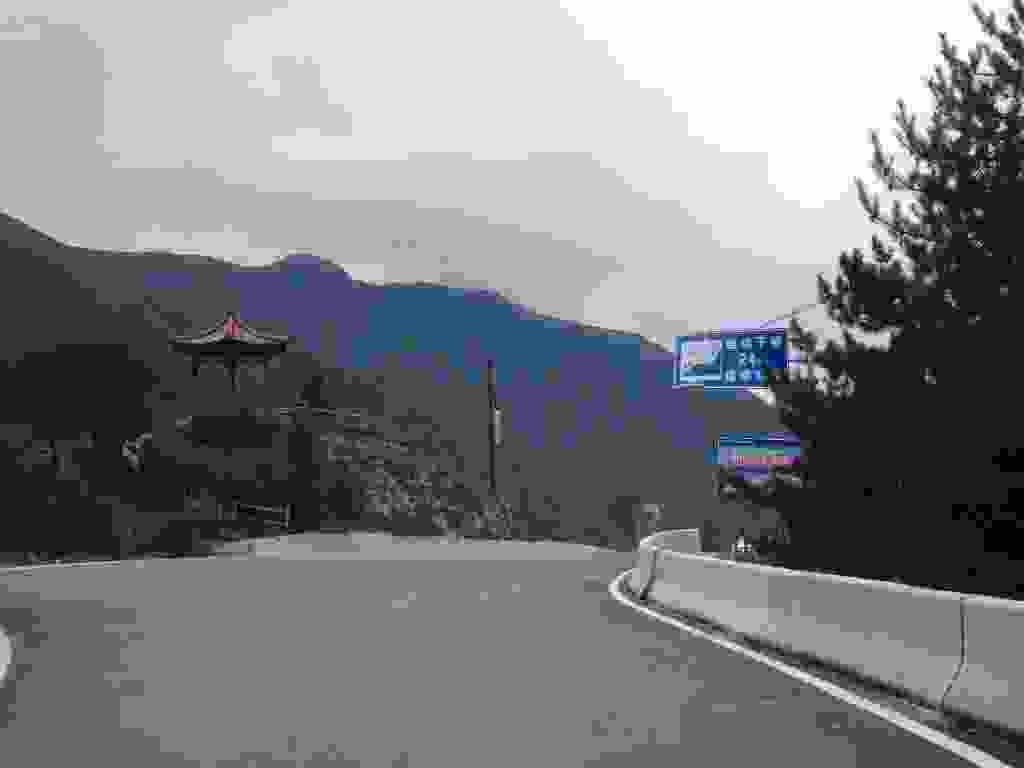
\includegraphics[width=\mywidth]{../wp-content/uploads/2015/09/wpid-p9136854-1024x768.jpg} \end{center}
\begin{center} 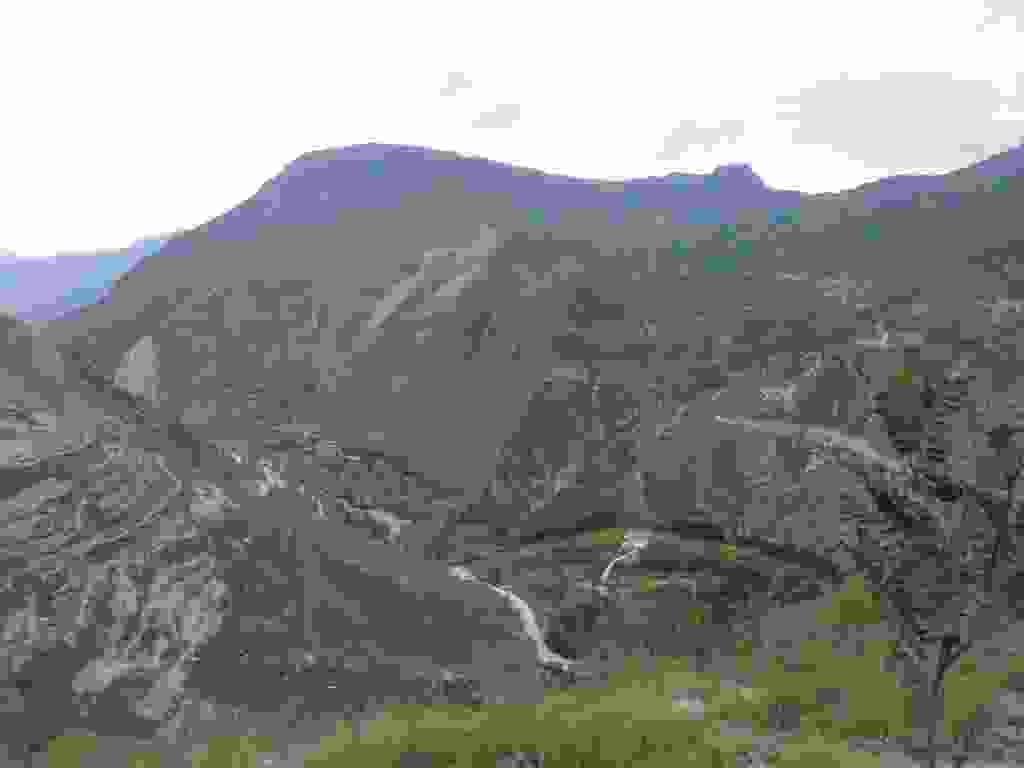
\includegraphics[width=\mywidth]{../wp-content/uploads/2015/09/wpid-p9136857-1024x768.jpg} \end{center}

 Le soleil fait son apparition le dernier jour. 
\begin{center} 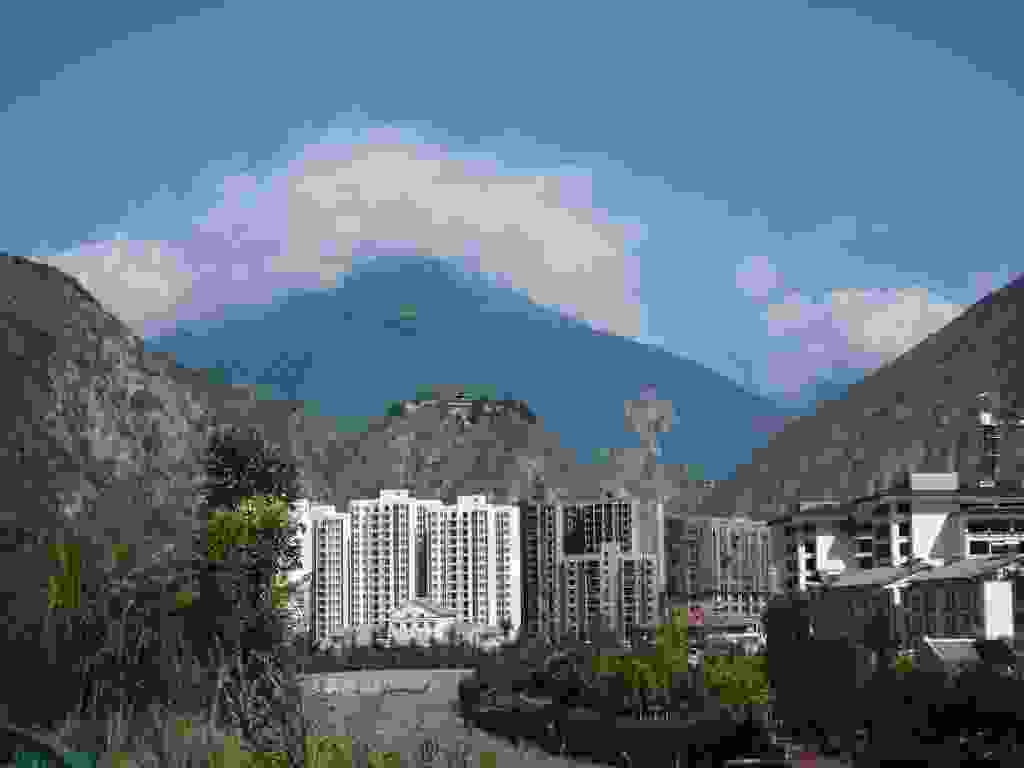
\includegraphics[width=\mywidth]{../wp-content/uploads/2015/09/wpid-p9146869-1024x768.jpg} \end{center}
\begin{center} 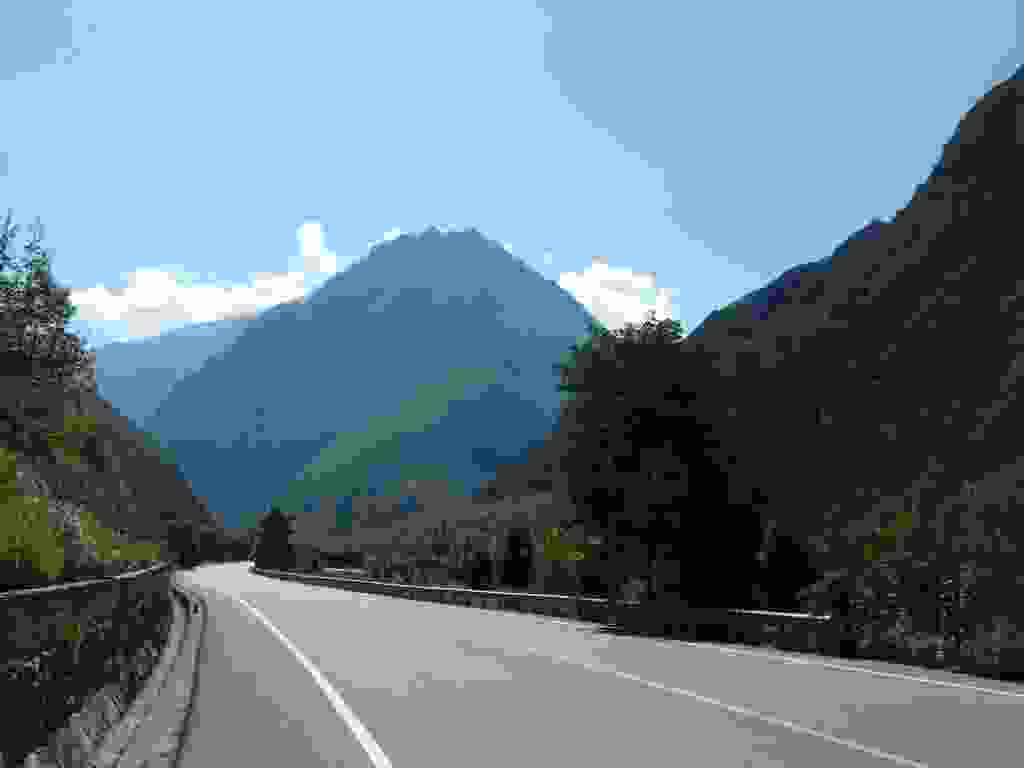
\includegraphics[width=\mywidth]{../wp-content/uploads/2015/09/wpid-p9146871-1024x768.jpg} \end{center}
